\RequirePackage{letltxmacro}
\LetLtxMacro{\LaTeXtextbf}{\textbf}
\documentclass{ieeeaccess}
\LetLtxMacro{\textbf}{\LaTeXtextbf}
\usepackage{cite}
\usepackage{amsmath,amssymb,amsfonts}
% \usepackage{algorithmicx}%
% \usepackage{algpseudocode}%
\usepackage{graphicx}
\graphicspath{{figures/}{photos/}{assets/}{fonts/}}
\usepackage{textcomp}
% \usepackage{xcolor}%
\usepackage{subcaption}
\usepackage{textcomp}%
\usepackage{manyfoot}%
\usepackage{booktabs}%
\usepackage{listings}%
\usepackage{url}
\usepackage{caption}
\usepackage{multirow}
\usepackage{hyperref}
\usepackage[ruled,vlined]{algorithm2e}
\usepackage{threeparttable}
\usepackage{pifont}

\newcommand{\cmark}{\ding{51}} % check mark
\newcommand{\xmark}{\ding{55}} % cross mark

\usepackage{bm}
\makeatletter
\AtBeginDocument{\DeclareMathVersion{bold}
\SetSymbolFont{operators}{bold}{T1}{times}{b}{n}
\SetSymbolFont{NewLetters}{bold}{T1}{times}{b}{it}
\SetMathAlphabet{\mathrm}{bold}{T1}{times}{b}{n}
\SetMathAlphabet{\mathit}{bold}{T1}{times}{b}{it}
\SetMathAlphabet{\mathbf}{bold}{T1}{times}{b}{n}
\SetMathAlphabet{\mathtt}{bold}{OT1}{pcr}{b}{n}
\SetSymbolFont{symbols}{bold}{OMS}{cmsy}{b}{n}
\renewcommand\boldmath{\@nomath\boldmath\mathversion{bold}}}
\makeatother

\def\BibTeX{{\rm B\kern-.05em{\sc i\kern-.025em b}\kern-.08em
    T\kern-.1667em\lower.7ex\hbox{E}\kern-.125emX}}

%Your document starts from here ___________________________________________________
\begin{document}
\history{Date of publication xxxx 00, 0000, date of current version xxxx 00, 0000.}
\doi{xx.xxxx/ACCESS.2026.xxxxxxx}

\title{Lightweight Data Augmentation Techniques for Imbalanced Learning}

\author{\uppercase{Thai-Duy Dinh}\authorrefmark{1},
\uppercase{Minh-Thuan Nguyen}\authorrefmark{1}, 
\uppercase{Thanh-Kim Le Duc}\authorrefmark{1},
\uppercase{Duc-Quang Vu}\authorrefmark{2},
\uppercase{Ngoc-Hoang Tran}\authorrefmark{3},
\uppercase{Anh-Cang Phan}\authorrefmark{4},
\uppercase{Ngoc-Hoang Le}\authorrefmark{7},
\uppercase{Phung-Anh Nguyen}\authorrefmark{6},
\uppercase{Tan-Ha Mai}\authorrefmark{5},
and \uppercase{Lam-Son L\^{e}}\authorrefmark{1} \IEEEmembership{Member, IEEE}}

\address[1]{Faculty of Engineering, Vietnamese-German University, Ho Chi Minh City 75911, Vietnam}
\address[2]{Faculty of Information Technology, Thai Nguyen University of Information and Communication Technology, Vietnam}
\address[3]{Department of Software Engineering, FPT University, Can Tho, Vietnam}
\address[4]{Vinh Long University of Technology Education, Vinh Long, Vietnam}
\address[5]{Department of Computer Science and Information Engineering, National Taiwan University, Taipei, Taiwan}
\address[6]{Graduate Institute of Data Science, Taipei Medical University, Taipei, Taiwan}
\address[7]{Graduate Institute of Biomedical Materials and Tissue Engineering, Taipei Medical University, Taipei, Taiwan}
%\tfootnote{This paragraph of the first footnote will contain support information, including sponsor and financial support acknowledgment.}

\markboth
{Author \headeretal: Preparation of Papers for IEEE Access}
{Author \headeretal: Preparation of Papers for IEEE Access}

\corresp{Corresponding author: Lam-Son L\^{e} (e-mail: son.ll@vgu.edu.vn).}


\begin{abstract}
Imbalanced learning, when some classes have far fewer examples than others, creates real challenges in areas like medical diagnosis, fraud detection, and rare-event forecasting. Advanced generative methods, such as GANs, diffusion models, and DeepSMOTE, can effectively augment minority-class examples, but typically demand substantial compute resources and complex pipelines, which limits their practicality in environments with limited resources. In this work, we focus instead on lightweight data-augmentation techniques that balance speed and accuracy. By combining simple augmentations (Mixup, Cutout) with careful resampling and class-weighting, we achieve significant gains in minority-class performance without extra computational cost. Evaluated on imbalanced versions of SVHN-10, CIFAR-10, CINIC-10, CIFAR-100 and TinyImageNet-200 our approach consistently improves both minority-class accuracy and overall generalization, while keeping training fast and resource-friendly. These results offer a practical solution to handling class imbalance in constrained environments. Our implementation is available as an open-source project on GitHub\footnote{\url{https://github.com/duydinhthai27/lightweight-ILWH}}.

\end{abstract}

\begin{keywords}
%Enter key words or phrases in alphabetical order, separated by commas. 
Deep Learning, Lightweight Data Augmentation, Imbalanced Classification, Imbalanced Lightweight Hybrid Approach.
\end{keywords}

\titlepgskip=-21pt

\maketitle


\section{Introduction}
% \ha{consider to structure as introduction format in Computer Science, you can consider to refer the introductio of this paper: \url{https://www.csie.ntu.edu.tw/~htlin/paper/doc/pakdd25aclimage.pdf}}
Imbalanced learning refers to scenarios where certain classes are significantly underrepresented compared to others in a dataset \cite{cao2019learning, cheng2023smote, vu2024lcsl, mai2025-icm, prototype-longtailed}.
This disparity can severely impact the performance of machine learning models, as they often become biased towards the majority class, leading to suboptimal predictions for the minority class. Such challenges are especially prevalent in critical domains like medical diagnosis, fraud detection, and rare event forecasting, where identifying the minority class accurately is of utmost importance \cite{krawczyk2016learning, he2009learning, le2024semantic}.

\begin{figure}[t]
    \centering
        \centering
        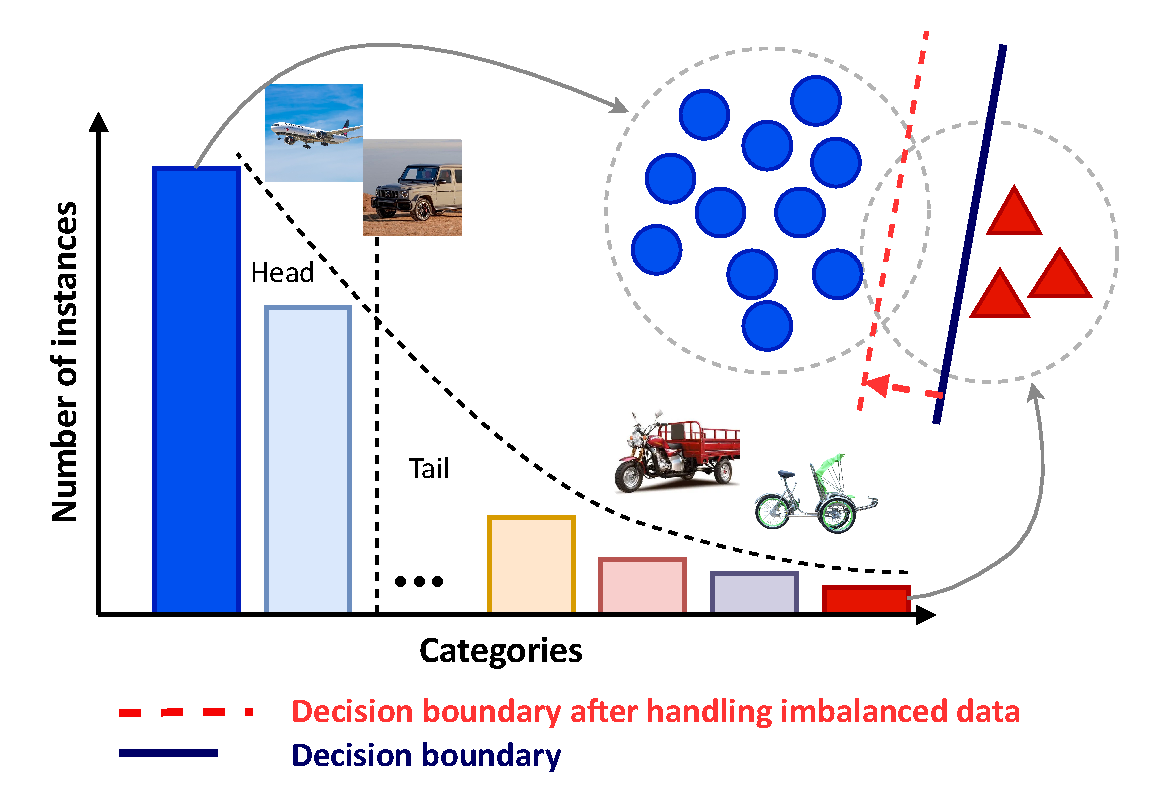
\includegraphics[width=\columnwidth]{imbalance-Page-2.drawio.pdf}
        \caption{Visualization of a long-tailed dataset distribution. The graph illustrates that certain categories, like airplanes and trucks, appear frequently in the dataset, while other less common or specialized vehicles, such as three-wheeled motorbike, occur much less often. This long-tailed distribution reflects real-world imbalances where some classes dominate, and many others have sparse representation.}
\label{fig:cifar10_imbalance_combined}
\end{figure}

Addressing imbalanced data requires strategies that can mitigate the inherent difficulties posed by skewed distributions. Traditional approaches fall broadly into three categories: data-level techniques, algorithm-level modifications, and hybrid methods \cite{sun2009classification, he2009learning}. Data-level techniques, such as oversampling and undersampling~\cite{unbiased_sample}, adjust the distribution by replicating minority class samples or reducing majority class samples. Algorithmic modifications, such as cost-sensitive learning, assign higher misclassification penalties to the minority class, thereby improving its representation during training. Hybrid approaches combine these strategies for enhanced performance. Prominent examples include Synthetic Minority Over-sampling Technique (SMOTE), ensemble-based methods, and cost-sensitive learning frameworks \cite{chawla2002smote, he2009learning}.

Recent advancements, such as  Margin-Aware Mixup (MAMix), have introduced Mixup-based data augmentation and adaptive learning strategies, significantly improving model generalization on imbalanced datasets \cite{cheng2023smote}. MAMix enhances minority class representations and mitigates decision boundary bias by dynamically adjusting Mixup parameters during training. Despite these developments, deep learning models remain vulnerable to class imbalance due to their dependency on large datasets and their tendency to amplify biases towards the majority class \cite{krawczyk2016learning}. This vulnerability underscores the need for more effective and computationally efficient solutions.
\textbf{Motivation.} While numerous techniques exist to address imbalanced learning, many involve a trade-off between computational efficiency, scalability, and model accuracy. Traditional resampling methods often require extensive parameter tuning and can be computationally intensive \cite{he2009learning}.
%Recent state-of-the-art methods such as Generative Adversarial Networks (GANs) have shown remarkable versatility and effectiveness in imbalanced learning \cite{yadav2025rebalancingscalessystematicmapping}, but they also face several long-standing challenges and limitations, such as excessive resource utilization and implementation constraints.
The field is bounded by resource-intensive deep learning on the end and less effective tuning-heavy traditional methods on the other. Between these two extremes lie the lightweight imbalanced learning techniques. They minimize computational overhead without sacrificing performance and are becoming increasingly critical, especially in resource-constrained environments such as Internet of Things (IoT) and edge devices.
%Techniques such as Mixup \cite{zhang2017Mixup}, when combined with Deferred Re-Weighting (DRW) schedules \cite{cao2019learning}, present promising alternatives by more effectively distributing the data during training and maintaining.
% \textbf{Fair Comparison and Lightweight Techniques.} To evaluate the effectiveness of lightweight strategies and sampling methods, it is essential to systematically analyze their impact on both computational efficiency and model performance. This involves considering trade-offs in time complexity, scalability, and classification accuracy. Such an analysis is particularly relevant for deep learning, where the issue of class imbalance is often magnified.
\texorpdfstring{\textbf{Objective.}}{Objective.}
Our objective is to identify
the most suitable augmentation approach for each specific
method, avoiding the extremes of underutilization and overutilization in ways that might introduce noise or degrade model performance. By systematically analyzing augmentation placement within the training pipeline, our objective is to develop a highly adaptive, context-aware augmentation strategy. The goal is to maximize generalization and performance in diverse machine learning applications.

\textbf{Contribution.} 
In this work, we focus on lightweight approaches to resolving class imbalance, with an emphasis on integrating Mixup with DRW schedules. By systematically comparing these methods across various resampling strategies, we demonstrate that combining Mixup and DRW achieves significant improvements in model performance while keeping the computational cost under control. This study contributes to advancing the state-of-the-art by providing scalable, robust solutions for imbalanced learning scenarios, where computing resources are under constraint. Moreover, we further investigate to determine the optimal timing and conditions for applying augmentation techniques. Understanding when and how to introduce data augmentation is crucial, as different augmentation strategies may yield varying levels of effectiveness depending on the dataset characteristics, model architecture, and training dynamics.

The remainder of this paper is organized as follows. Section~\ref{sec:related_work} reviews prior work in the field. In Section~\ref{sec:motivation}, we present the motivation for adopting lightweight techniques. Our proposed methodology is detailed in Section~\ref{sec:methodology}. We describe our experimental setup in Section~\ref{sec:experiments}, present our main results and a detailed ablation study in Section~\ref{sec:ablation}, and conclude in Section~\ref{sec:conclusion}.
\section{Related Work} \label{sec:related_work}
% \ha{long-tailed}
\subsection{Problem Setup}
We begin by reviewing the problem formulation for imbalanced multi-class classification. We consider the imbalanced $K$-class classification problem, where $K > 2$. Given a training dataset $\mathcal{D} = \{(\mathbf{x}_1, y_1), \dots, (\mathbf{x}_n, y_n)\}$, each input $\mathbf{x}_i \in \mathcal{X} \subseteq \mathbb{R}^d$ represents a feature vector, and its corresponding label $y_i \in \mathcal{Y} \subseteq \mathbb{R}^K$ is drawn from the joint distribution $P_{\mathbf{x}, y}^{\text{all}}$. The objective is to learn a classifier $f_{\mathbf{x}} \colon \mathbb{R}^d \to \mathbb{R}^K$ that minimizes the standard loss function:  
$L(\theta) = \mathbb{E}_{\mathbf{x}, y \sim P_{\mathbf{x}, y}^{\text{all}}} [\ell(f(\mathbf{x}), y)],$
where $\ell(\cdot, \cdot)$ is a predefined loss function, and $e_y$ denotes the one-hot encoded vector corresponding to label $y$. The predicted label $\hat{y}$ for an instance $\mathbf{x}$ is determined using the argmax function:  
$\hat{y} = \mathop{\arg\max}_{k \in K} f(\mathbf{x})_k,$
where $f(\mathbf{x})_k$ is the $k^{\text{th}}$ component of the output of $f(\mathbf{x})$.  
Let $n_j$ denote the size of class $j$. We assume the training dataset is \textit{imbalanced}, meaning the size of the largest class, $\max_i n_i$, differs significantly from that of the smallest class, $\min_i n_i$. The \textit{class imbalance ratio}, $\rho$, quantifies the degree of imbalance and is defined as:  
$\rho = \max_i n_i / \min_i n_i.$
This ratio serves as a measure of the imbalance of the dataset, with larger $\rho$ values indicating greater imbalance. In this context, the larger classes are referred to as the \emph{majority}, while the smaller ones are termed the \emph{minority}.  
After training $f(\mathbf{x})$ on the \textit{imbalanced} dataset, we follow the evaluation procedure outlined in~\cite{cao2019learning, cheng2023smote}. Specifically, the classifier is tested on a \textit{balanced} test set generated from the same conditional distribution $P(\mathbf{x} \mid y)$ for each class. This evaluation approach ensures equal importance is given to each class during testing, providing a fair assessment of the classifier's performance across all classes.
%%%% HA comment 22 Oct, 2025
% \textbf{Hybrid approaches} combine data-level and algorithm-level strategies to leverage the strengths of both and achieve more robust performance. These methods often integrate resampling techniques directly into the training process of an algorithm. For example, a popular hybrid strategy involves combining sampling methods with ensemble learning, such as creating balanced data subsets for each learner in a bagging or boosting framework.

\subsection{Imbalanced Learning Approaches}
\label{Mixup_interpolation}
To address the challenges, traditional solutions are broadly categorized into two families: \textit{data-oriented approaches} and \textit{algorithm-oriented approaches}.

% \textbf{Data-oriented approaches} directly address class imbalance by manipulating the training dataset itself to create a more balanced distribution. This is typically achieved by either oversampling the minority class to increase its representation or undersampling the majority class to reduce its dominance. Techniques range from simple random replication to more sophisticated synthetic sample generation methods like the SMOTE \cite{chawla2002smote}, which creates new minority instances by interpolating between existing ones.

% \textbf{Algorithm-oriented approaches}, in contrast, modify the learning algorithm to be more sensitive to the minority class without altering the training data. The most common strategy is cost-sensitive learning, which adjusts the model's objective function to assign higher misclassification penalties to errors made on minority class instances. This forces the model to prioritize learning the characteristics of underrepresented classes, effectively shifting the decision boundary to improve their recognition.

\paragraph{Data-oriented approaches} At the data level, methods reshape the training distribution to alleviate imbalance prior to optimization. While SMOTE \cite{chawla2002smote} remains a cornerstone, many extensions improve sample quality and coverage. For instance, k-Means SMOTE \cite{douzas2018improving} synthesizes minority examples within cluster-consistent regions, and reinforcement learning–based resampling \cite{fan2021imbalanced} adaptively selects/weights samples to maximize downstream accuracy. Beyond pure resampling, data augmentation has proven especially effective. Mixup \cite{zhang2017Mixup} constructs virtual examples by linearly interpolating pairs of inputs and labels, encouraging smoother decision boundaries and reducing overfitting to majority classes. These examples are generated via simple linear combinations as follows:

\begin{equation}
\label{mixup_x}
\tilde{\mathbf{x}} = \lambda \mathbf{x}_i + (1 - \lambda) \mathbf{x}_j,
\end{equation}
\begin{equation}
\label{mixup_y}
\tilde{y} = \lambda y_i + (1 - \lambda) y_j,
\end{equation}
where: \( (\mathbf{x}_i, y_i) \) and \( (\mathbf{x}_j, y_j) \) are two examples drawn from the training data using a sampling strategy (e.g., uniform, class-weighted, or oversampling). $\lambda \sim \mathit{Beta}(\gamma, \gamma)$ distribution.
\begin{figure}[htb]
    \centering
        \centering
        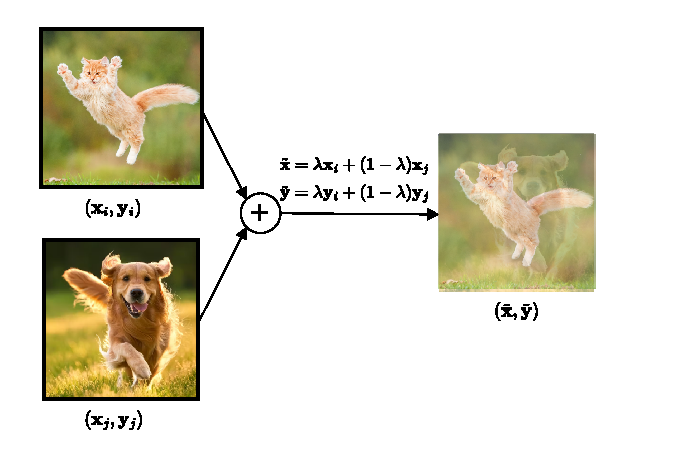
\includegraphics[width=0.9\columnwidth]{imbalanced.pdf}
        \caption{Illustration of the Mixup data augmentation technique. Two training samples 
     $(x_i, y_i)$ and $(x_j, y_j)$ are linearly combined with a mixing coefficient 
    $\lambda_x \sim \mathit{Beta}(\gamma, \gamma)$\ to generate a new virtual sample $(\tilde{x}, \tilde{y})$.}
\label{fig:cifar10_imbalance_mixup}
\end{figure}

By incorporating different sampling methods, such as class-weighted or oversampling, the technique ensures that underrepresented classes are more frequently sampled, mitigating the impact of class imbalance. Sampling-based Mixup has been shown to enhance the diversity of training data, reduce the memorization of corrupt labels, improve robustness to adversarial training, and boost the generalizability of deep networks. This approach is particularly beneficial for tasks with severe class imbalance, leading to improved performance across a variety of image classification tasks.

\paragraph{Algorithm-Oriented Approaches} Algorithm-level strategies modify the learning objective or training schedule to account for imbalance without changing the data. Cost-sensitive learning has progressed beyond fixed class weights. For classical models, Automatically Tuning the Error Cost (ATEC) \cite{cao2020expediting} adapts misclassification penalties for SVMs; for fast-training neural architectures, DKWBLS \cite{chen2022double} incorporates explicit class-dependent weighting. Ensemble methods remain strong—beyond RUSBoost \cite{seiffert2009rusboost}, newer variants (e.g., ECUBoost \cite{wang2020entropy} and SMOTEWB \cite{saglam2022novel}) integrate uncertainty-aware undersampling or noise-aware boosting. In deep long-tailed recognition, a dominant line uses re-weighting by the effective number of samples \cite{cui2019classbalanced} and margin-adjusted objectives such as LDAM \cite{cao2019learning}. Deferred Re-Weighting (DRW) \cite{cao2019learning} operationalizes this by first learning representations on the original (imbalanced) data and then activating class-balanced weights later in training to avoid early overfitting to rare classes. This approach first trains the model on the original imbalanced data for a set number of epochs to learn general representations and only then introduces class-balancing weight. This delay prevents the model from overfitting to the minority classes early in training.

The re-weighting in DRW is guided by the concept of the effective number of samples, which accounts for the diminishing marginal value of additional examples within the same class \cite{cui2019classbalanced}. In lieu of using the raw sample count \(n_c\), this approach recognizes that new samples in overrepresented classes often contribute redundant information. The effective number $E_{n_c}$ for a class $c$ with $n_c$ samples is defined as:
\begin{equation}
E_{n_c} = \frac{1 - \beta^{n_c}}{1 - \beta}, \quad \beta \in [0, 1)
\end{equation}
here, $\beta$ is a hyperparameter that controls the decay rate, with larger values emphasizing rare classes better. The corresponding weight for class $c$ is:
\begin{equation}
w_c = \frac{1 - \beta}{1 - \beta^{n_c}}
\end{equation}
This formulation provides a theoretically grounded method to balance classes in the loss function by incorporating sample informativeness rather than raw frequency.
% At the data level, while SMOTE \cite{chawla2002smote} remains a foundational method, recent works have introduced more advanced variants. For instance,  \cite{douzas2018improving} proposed k-means SMOTE to improve the quality of synthetic samples by clustering the data first. Other modern approaches integrate sophisticated learning paradigms, such as the work by Fan et al. (2021), which employs a deep reinforcement learning algorithm to optimize the sample selection and distribution strategy \cite{fan2021imbalanced}.

% On the algorithm level, cost-sensitive learning has evolved beyond simple weighting schemes. \cite{cao2020expediting} developed Automatically Tuning the Error Cost (ATEC), an adaptive error cost adjustment method for Support Vector Machines (SVMs) that automatically tunes misclassification costs to enhance performance without expensive grid searches \cite{cao2020expediting}. In the context of shallow neural networks, recent methods like the Double-Kernelized Weighted Broad Learning System (DKWBLS) have been proposed to explicitly handle class imbalance and improve decision boundaries in fast-training architectures \cite{chen2022double}.

% Ensemble methods remain a powerful and popular approach. Beyond classic algorithms like Random UnderSampling Boosting (RUSBoost) \cite{seiffert2009rusboost}, contemporary research has focused on creating more dynamic and robust ensembles. For example, Wang et al. (2020) introduced Entropy and Confidence-based Undersampling Boosting (ECUBoost), a framework that combines entropy and confidence-based undersampling within the boosting process to better preserve the structural distribution of the majority class \cite{wang2020entropy}. Hybrid methods also continue to advance, such as the Synthetic Minority Oversampling Technique with Weighted Boosting (SMOTEWB) technique, which combines a novel noise detection method with boosting to overcome the limitations of random oversampling \cite{saglam2022novel}.

% With the advent of deep learning, the challenge is often framed as long-tail learning. A dominant strategy in this area involves re-weighting the loss function based on the ``effective number of samples'', which accounts for data overlap and diminishing returns from additional examples \cite{cui2019classbalanced}. This principle is central to influential loss functions like the Label-Distribution-Aware Margin (LDAM) loss \cite{cao2019learning}. A significant paradigm shift was introduced with decoupled training, which proposes a two-stage process: learning feature representations on the original imbalanced data, and then training only the classifier on a class-balanced subset \cite{kang2019decoupling}. This approach has proven highly effective and has inspired numerous follow-up works. Other deep learning solutions adapt data-level ideas, such as DeepSMOTE, which fuses an encoder-decoder framework with SMOTE-based oversampling \cite{dablain2022deepsmote}.

% While these state-of-the-art methods demonstrate strong performance, they often rely on computationally intensive training schemes, complex loss formulations, or multi-stage pipelines. Our work diverges from this trend by focusing on lightweight, computationally efficient data augmentation and sampling techniques that can be seamlessly integrated into standard training loops to effectively address class imbalance with minimal overhead.

% \subsection{Mixup}
% \label{Mixup_interpolation}
% One of the most effective regularization—or data augmentation—techniques in deep neural networks for image classification is Mixup, which can be adapted to leverage different sampling methods for constructing virtual training examples. These examples are generated via simple linear combinations as follows:

% \begin{equation}
% \label{mixup_x}
% \tilde{\mathbf{x}} = \lambda \mathbf{x}_i + (1 - \lambda) \mathbf{x}_j,
% \end{equation}
% \begin{equation}
% \label{mixup_y}
% \tilde{y} = \lambda y_i + (1 - \lambda) y_j,
% \end{equation}

% where:
% \begin{itemize}
%     \item \( (\mathbf{x}_i, y_i) \) and \( (\mathbf{x}_j, y_j) \) are two examples drawn from the training data using a sampling strategy (e.g., uniform, class-weighted, or oversampling).
%     \item $\lambda \sim \mathit{Beta}(\gamma, \gamma)$ distribution.
% \end{itemize}
% \begin{figure}[htb]
%     \centering
%         \centering
%         \includegraphics[width=0.45\textwidth]{src/chart/imbl (3).pdf}
%         \caption{Illustration of the Mixup data augmentation technique. Two training samples 
%      $(x_i, y_i)$ and $(x_j, y_j)$ are linearly combined with a mixing coefficient 
%     $\lambda_x \sim \mathit{Beta}(\gamma, \gamma)$\ to generate a new virtual sample $(\tilde{x}, \tilde{y})$.}
% \label{fig:cifar10_imbalance_combined}
% \end{figure}
% By incorporating different sampling methods, such as class-weighted or oversampling, the technique ensures that underrepresented classes are more frequently sampled, mitigating the impact of class imbalance. Sampling-based Mixup has been shown to enhance the diversity of training data, reduce the memorization of corrupt labels, improve robustness to adversarial training, and boost the generalizability of deep networks. This approach is particularly beneficial for tasks with severe class imbalance, leading to improved performance across a variety of image classification tasks.

% \subsection{Deferred Re-Weighting (DRW)}
% A prominent and successful algorithm-level strategy is DRW, a two-stage training schedule that balances classes in the loss function by incorporating sample informativeness rather than raw frequency \cite{cao2019learning}. This approach first trains the model on the original imbalanced data for a set number of epochs to learn general representations and only then introduces class-balancing weight. This delay prevents the model from overfitting to the minority classes early in training.

% The re-weighting in DRW is guided by the concept of the effective number of samples, which accounts for the diminishing marginal value of additional examples within the same class \cite{cui2019classbalanced}. In lieu of using the raw sample count \(n_c\), this approach recognizes that new samples in overrepresented classes often contribute redundant information. The effective number $E_{n_c}$ for a class $c$ with $n_c$ samples is defined as:
% \begin{equation}
% E_{n_c} = \frac{1 - \beta^{n_c}}{1 - \beta}, \quad \beta \in [0, 1)
% \end{equation}
% here, $\beta$ is a hyperparameter that controls the decay rate, with larger values emphasizing rare classes better. The corresponding weight for class $c$ is:
% \begin{equation}
% w_c = \frac{1 - \beta}{1 - \beta^{n_c}}
% \end{equation}
% This formulation provides a theoretically grounded method to balance classes in the loss function by incorporating sample informativeness rather than raw frequency.
%%%% HA comment 22 Oct, 2025
% In our work, we adopt the effective number to guide both the loss function and sampling strategies. Specifically, the weight $w_c$ is  used to: 
% (1) Re-Weight the loss function in the second phase of DRW schedule~\cite{cao2019learning}, which prevents early overfitting to minority classes by delaying the re-weighting mechanism. (2) Initialize sampling probabilities in both the \textit{Weighted Random Batch Sampler (WRBS)} and \textit{Weighted Fixed Batch Sampler (WFBS)} modules. This ensures more consistent and meaningful exposure to minority class samples throughout training.
%%%% HA comment 22 Oct, 2025
% Moreover, the integration of the effective number with \textit{Mixup-based augmentation} is particularly beneficial. While Mixup generates interpolated data to smooth class boundaries, the effective number ensures that underrepresented classes contribute proportionally more to the loss. This dual mechanism improves model generalization under heavy imbalance while maintaining computational efficiency. Although the effective number is commonly used in heavy-weight deep learning pipelines, our study demonstrates its viability in lightweight frameworks, making it suitable for resource-constrained applications such as edge computing or embedded systems.
\section{Motivation for Lightweight Imbalance Techniques} \label{sec:motivation}
% Imbalanced class distributions pose a persistent challenge in machine learning, especially for multi-class classification. A wealth of sophisticated methods have been proposed to improve learning from imbalanced data \cite{Chen2024,Ghosh2024}.
% %These include data-level techniques (\textit{e.g. complex oversampling and undersampling schemes}), algorithm-level strategies (\textit{cost-sensitive learning that adjusts class weight in the loss function}), advanced ensemble methods (\textit{bagging/boosting ensembles tailored to imbalance}), and specialized deep long-tail recognition networks \cite{Chen2024}. 
% While such state-of-the-art approaches can boost minority-class accuracy, they typically do so at the expense of high computational cost and added complexity. For example, boosting-based ensemble solutions must train many weak learners in sequence; this iterative process significantly increases training time and resource requirements, especially on large datasets. Chen et al. \cite{Chen2024} observe that although ensembles improve performance, a notable drawback of methods like AdaBoost is the “relatively higher computational cost” due to multiple training iterations and updates, which can render them impractical for large-scale tasks. 

% Similarly, deep cost-sensitive models require careful tuning of class weight hyperparameters or modified loss functions, and achieving the right balance can be complex. Long-tailed recognition networks (\textit{designed for extreme class imbalance}) often introduce additional network branches or expert subnetworks to better learn tail classes. 
% %A prominent example is the Bilateral-Branch Network (BBN) , which trains separate feature extractor and classifier branches for head and tail classes \cite{Ghosh2024}. Such architectures improve recognition of rare classes but substantially increase model size and training complexity. Likewise, generative oversampling methods train auxiliary generative models (\textit{e.g. GAN-based synthetic data generation}) to augment minority classes. 
% Although effective in certain cases, these generative approaches add considerable overhead. Ghosh et al. \cite{Ghosh2024} highlight that many GAN-based oversampling techniques suffer from slow training due to the extra computations (\textit{for instance, computing nearest neighbors in each mini-batch to generate new samples}), which can significantly slow down learning on large-scale problems. 
%In summary, the latest surveys \cite{Chen2024,Ghosh2024} concur that many cutting-edge imbalance solutions—ensemble frameworks, deep cost-sensitive algorithms, long-tail networks, and generative data augmenters—tend to be resource-intensive, with complex designs that may yield diminishing returns relative to their computational expense. Indeed, Chen et al. \cite{Chen2024} note that such methods often exhibit “high computational complexity, complex model design, and no guaranteed substantial improvements”, underscoring the need for more efficient alternatives. 


While a wealth of sophisticated methods have been proposed to improve learning from imbalanced data, state-of-the-art approaches often boost minority-class accuracy at the expense of high computational cost and added complexity. For example, boosting-based ensembles must train many weak learners in sequence, a process that significantly increases training time and resource requirements. Chen et al. \cite{Chen2024} note that this \textit{relatively higher computational cost} can render such methods impractical for large-scale tasks.

\begin{figure*}[t]
\centering
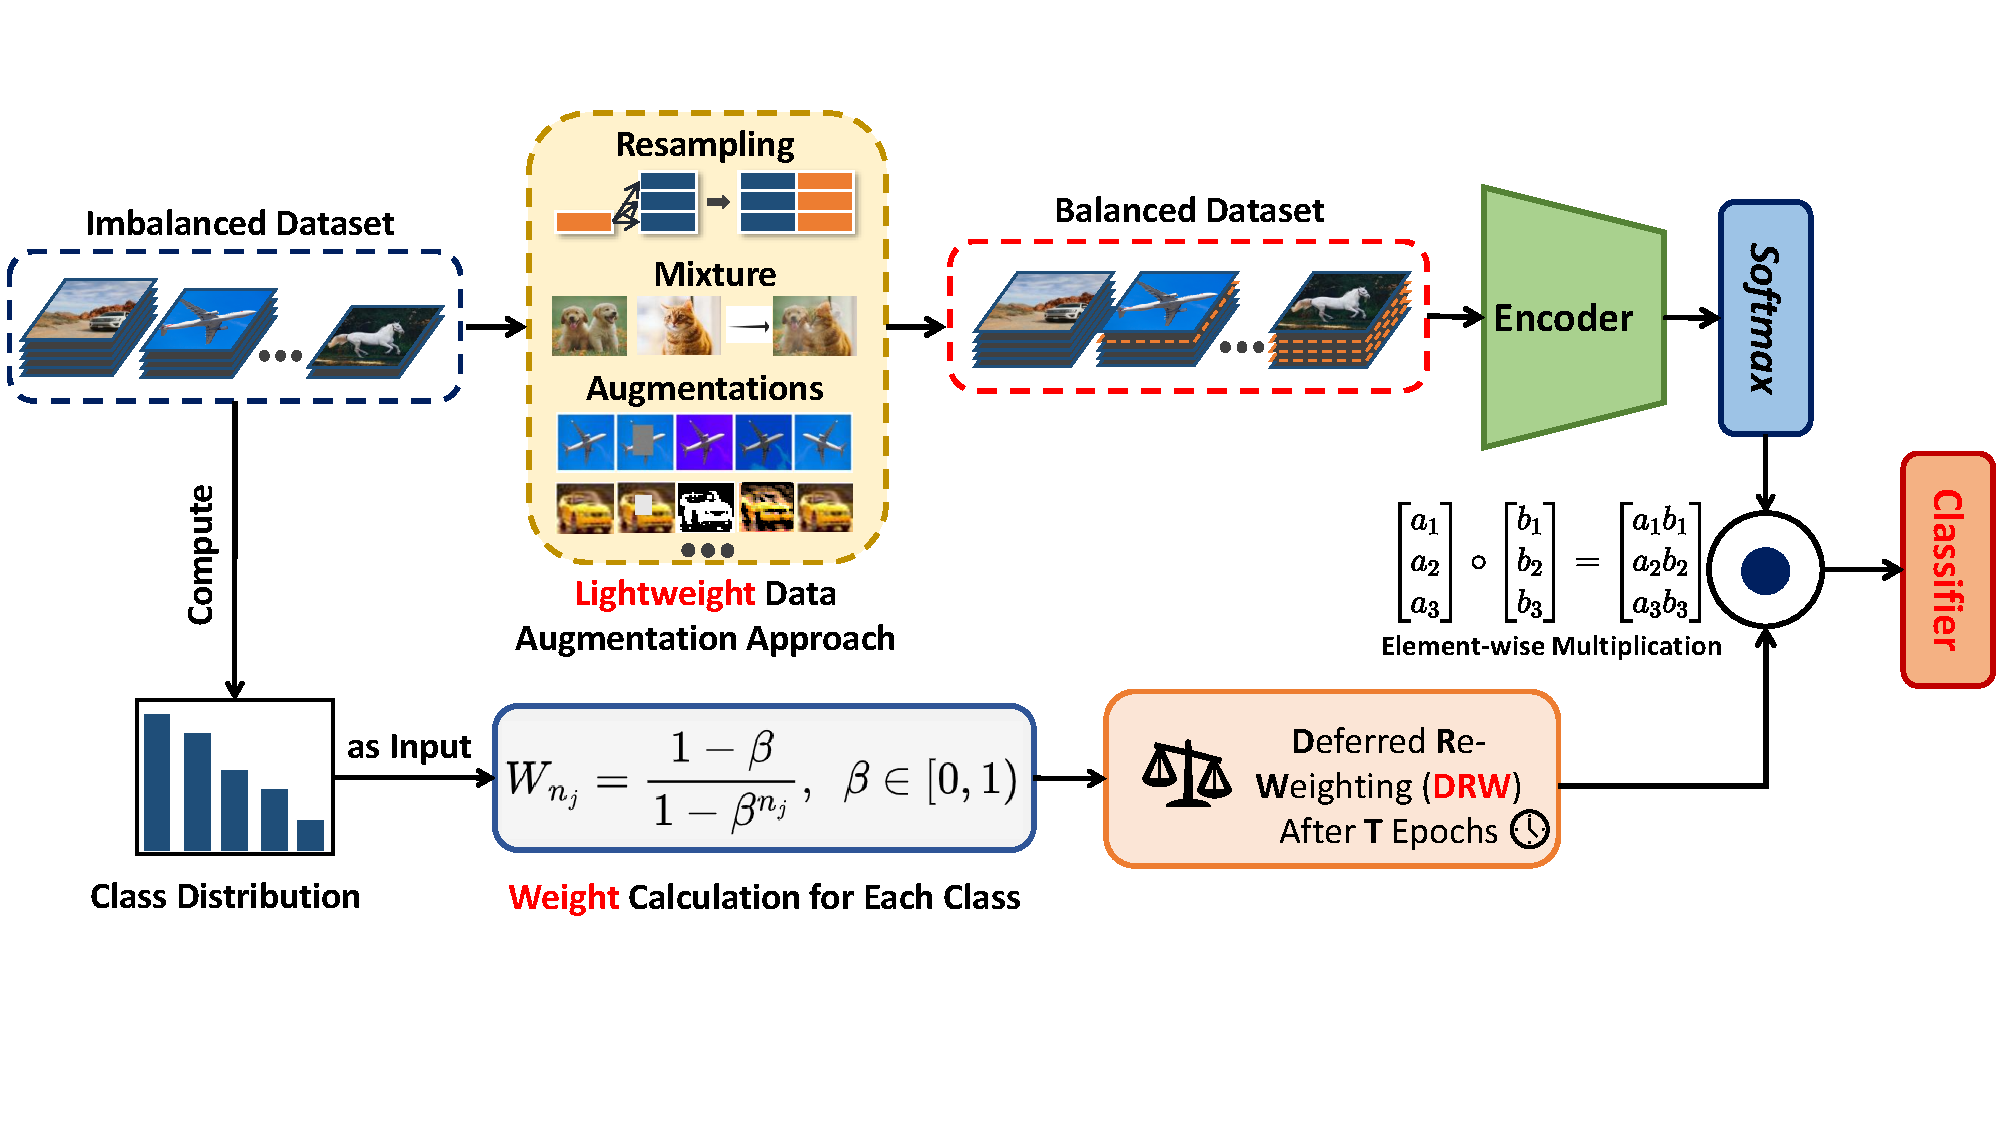
\includegraphics[width=\textwidth, clip, trim=0cm 2.5cm 0cm 1.5cm]
{Imbalanced-final}
    \caption{An overview of lightweight data augmentation techniques for imbalance learning.}
    \label{fig:imbalance_learning}
\end{figure*}

Similarly, other strategies incur significant overhead due to complex designs or auxiliary modules. Generative approaches like DeepSMOTE~\cite{dablain2022deepsmote}, which uses an encoder-decoder to synthesize minority samples, can lead to a computational overhead of 1.5 to 2 times the baseline cost. Ghosh et al. \cite{Ghosh2024} highlight that many GAN-based techniques suffer from slow training due to extra computations, such as finding nearest neighbors to generate new samples. Other methods, like MAMix~\cite{cheng2023smote}, introduce adaptive controllers that can increase training time by 15–25\%. In contrast, some techniques demonstrate that performance gains are possible without a heavy price; for instance, LDAM-DRW~\cite{cao2019learning} modifies a deferred class weighting schedule and adds negligible cost relative to standard training.
% \ha{consider putting a clock to signify a delay}

These concerns motivate the adoption of lightweight techniques for class imbalance, which aim to rebalance learning at much lower computational cost. Rather than fundamentally altering the model architecture or training an army of classifiers, lightweight methods adjust the data seen by a standard model in simple but effective ways~\cite{lightweight-longtailed, lightweightfightingmodel}. Two widely practiced families of such techniques are data augmentation and sample weighting/sampling strategies. Data augmentation inflates the effective training set by applying label-preserving transformations to input examples, thereby improving generalization for minority classes without collecting new data. Notably, modern augmentation policies like AutoAugment \cite{cubuk2018autoaugment} and RandAugment \cite{cubuk2019randaugment} can be plugged into training pipelines to automatically generate diverse image variants. 
%(\textit{through random crops, flips, color jittering, rotations, etc.}) with virtually no additional model overhead. These methods require only minor computational effort for image transformations, yet can substantially enrich the variability of rare class samples. Likewise, simple augmentation tricks such as Cutout \cite{devries2017cutout} help the model learn more robust features for all classes, including the minority ones, without any increase in model parameters. Because augmentation operations are performed on-the-fly on the CPU/ GPU during data loading, they are highly efficient and scalable. In imbalanced settings, augmentation can be particularly beneficial when applied more aggressively to minority class examples, effectively boosting their presence. For instance, recent studies have explored the enhancement of majority class samples and transferring them to enrich minority classes, as well as learning augmentation policies tailored to long-tailed distributions (\textit{to avoid simply magnifying the imbalance}) \cite{Chen2024}. 
Overall, data augmentation offers a lightweight, domain-agnostic tool to improve class balance: one can obtain significant gains in minority-class recognition by simply leveraging existing images more effectively, rather than training complex new models. 

Another efficient remedy to imbalance is to adjust the sampling or weighting of training examples, so that minority classes are seen more frequently by the learner. Many deep learning pipelines support weighted random sampling, wherein each data instance is sampled with probability inversely proportional to its class frequency. This yields mini-batches that are approximately class-balanced on average, without altering the model itself. Implementing such a scheme is straightforward and incurs negligible overhead beyond the bookkeeping of sample weight. 
% \ha{shall we do font change to WeightedRandomBatchSample, WeightedFixedBatchSample and the like} 
A related technique is to use a fixed sampling ratio per class and tune a parameter $\alpha$ that controls how strongly the sampling favors minority classes. A small $\alpha$ might slightly up-sample rare classes, whereas a larger $\alpha$ moves closer to fully balanced sampling. By varying $\alpha$, one can smoothly trade off between biasing towards the minority class vs. preserving the original data distribution. Importantly, these sampling strategies are easy to integrate into training loops and avoid the need for any additional model training. They essentially reallocate existing data resources in a smarter way. Crucially, such data rebalancing can be combined with data augmentation for compound effect: e.g., one might oversample the rare classes and apply stronger augmentation to them, yielding a diverse set of synthetic minority examples at very low cost. Unlike generate new samples or fine-tuning a complicated cost-sensitive loss schedule, sampling and augmentation methods keep the training pipeline simple and computationally cheap. 

While both Mixup and Deferred Re-Weighting (DRW) have been extensively studied, our proposed Imbalanced Lightweight Hybrid (ILWH) introduces a distinct integration of these two paradigms within a unified, resource-efficient framework. Below, we outline the conceptual and practical distinctions between ILWH and related approaches such as MAMix, DeepSMOTE, and LDAM-DRW.

% Existing imbalance-handling strategies often incur significant additional computation due to complex model designs or auxiliary optimization modules. 
% DeepSMOTE~\cite{dablain2022deepsmote}, for example, employs an encoder--decoder generator to synthesize minority samples in latent space, leading to a computational overhead of approximately $1.5\times$ to $2\times$ the baseline cost. 
% MAMix~\cite{cheng2023smote} introduces an adaptive margin controller that dynamically adjusts interpolation ratios, resulting in a reported $15$--$25\%$ increase in training time. 
% In contrast, LDAM-DRW~\cite{cao2019learning} modifies only the deferred class weighting schedule and therefore adds negligible cost ($<5\%$) relative to standard Empirical Risk Minimization (ERM).
% Beyond their elegance and ease of implementation, lightweight imbalance techniques have demonstrated competitive performance in practice. On standard vision benchmarks with many classes — such as CIFAR-10, CIFAR-100, and SVHN — simple oversampling or class-balanced sampling strategies, together with appropriate augmentations, often close much of the accuracy gap between minority and majority classes. For example, on long-tailed versions of CIFAR, balancing the mini-batches by oversampling the scarce classes can markedly improve minority-class recall, sometimes rivaling the results of far more elaborate algorithms. Likewise, applying AutoAugment or RandAugment policies has been shown to boost overall accuracy on imbalanced CIFAR-100 with minimal tuning, nearly matching specialized long-tail methods in some studies. Indeed, an influential work by Kang et al. (2019) found that a relatively simple two-phase training (first learning a feature backbone on the natural imbalanced data, then re-training the classifier with class-balanced sampling) achieved state-of-the-art results on long-tailed recognition benchmarks, highlighting that complex imbalanced-learning machinery is not always necessary. This insight, echoed by Ghosh et al. \cite{Ghosh2024}, reinforces the appeal of lightweight solutions: they can yield robust models that perform well across all classes without the burden of extensive additional computation. In scenarios where computing resources are limited — e.g. deploying models on mobile, edge, or embedded devices — such efficient techniques are particularly attractive. A mobile or IoT device may not accommodate large ensemble models or GAN generators, but can readily handle a bit of extra data augmentation or a modified sampling scheme during training. By adopting these resource-friendly methods, one can mitigate class imbalance while keeping the model lean and the training requirements modest.

In summary, the high cost and complexity of many modern imbalance-learning algorithms motivate a turn towards lightweight alternatives that are easier to deploy and scale. 
%Data augmentation and smart sampling are two pillars of this approach, offering significant practical benefits: they are simple to implement, impose minimal computational overhead, and yet substantially improve model fairness and accuracy across classes. 
%Equally important, they integrate seamlessly into existing training pipelines on common datasets (\textit{such as CIFAR-10, CIFAR-100, CINIC-10, SVHN-10, TinyImageNet-200}) and do not require specialized architectures or costly procedures. This makes them ideal for researchers and practitioners aiming to address class imbalance under real-world constraints. 
The evidence so far suggests that these lightweight methods can performance competitiveness with far more complex techniques \cite{Chen2024,Ghosh2024}, striking an excellent balance between effectiveness and scalability. Therefore, it is highly compelling to leverage such approaches for imbalanced multi-class classification problems, particularly when working in resource-constrained environments or seeking broadly applicable, easy-to-tune solutions. We build on this motivation and advocate for imbalance mitigation strategies that remain accessible and computationally light-weight, without sacrificing too much in terms of accuracy.

\section{Lightweight Methods for Imbalanced Learning} \label{sec:methodology}

The proposed pipeline presents a novel approach to address class imbalance in machine learning. The process begins with the input of raw training data, which undergoes augmentation through a series of lightweight transformation techniques. 
%These techniques, including AutoRand, RandAug, Cutout, Mixup, and Sampling, generate diverse and representative training samples, ensuring that underrepresented classes receive adequate exposure during training. This enhancement step is crucial for reducing the bias inherent in unbalanced datasets, where certain classes have far more data than others.
% \ha{\textcolor{blue}{(RESOLVED) I temporarily leave the draft idea of our imbalanced learning method here. PLEASE HELP TO POLISH AND IMPROVE THE APPEARANCE OF IT !!!!}}
%Data augmentation leads to a more useful enriched training dataset, which serves as input for the imbalance learning phase.
In the learning stage, various strategies, such as reweighting, resampling, or class-balanced loss functions, can be applied to further enhance the performance of the model in minority classes. This step is critical in ensuring that the model does not simply memorize the majority class patterns but learns to generalize effectively across all categories. Finally, the trained model proceeds to the prediction phase, where it makes informed decisions based on the improved training distribution. The proposed ILWH combines Mixup-based sample interpolation with deferred re-weighting in a unified and lightweight manner. 
Since Mixup operates as a simple linear combination of input pairs within each mini-batch, it requires no auxiliary networks or additional forward--backward passes. 
Consequently, ILWH introduces less than $3\%$ runtime overhead compared to the ERM baseline, consistent with previous findings that Mixup-style methods are computationally efficient \cite{zhang2017Mixup}. 
Moreover, ILWH maintains the same number of trainable parameters as the backbone classifier, confirming that the method is structurally lightweight.

%This approach is motivated by the limitations of traditional imbalance-handling techniques, such as oversampling and cost-sensitive learning, which often introduce computational overhead or lead to overfitting. Unlike these conventional methods, lightweight data augmentation techniques offer an adaptive and computationally efficient solution to class imbalance. By introducing synthetic diversity, augmentations such as Mixup and RandAug prevent models from overfitting to specific class distributions and help smooth decision boundaries, thereby improving generalization.
\begin{figure}[htbp]
    \centering
    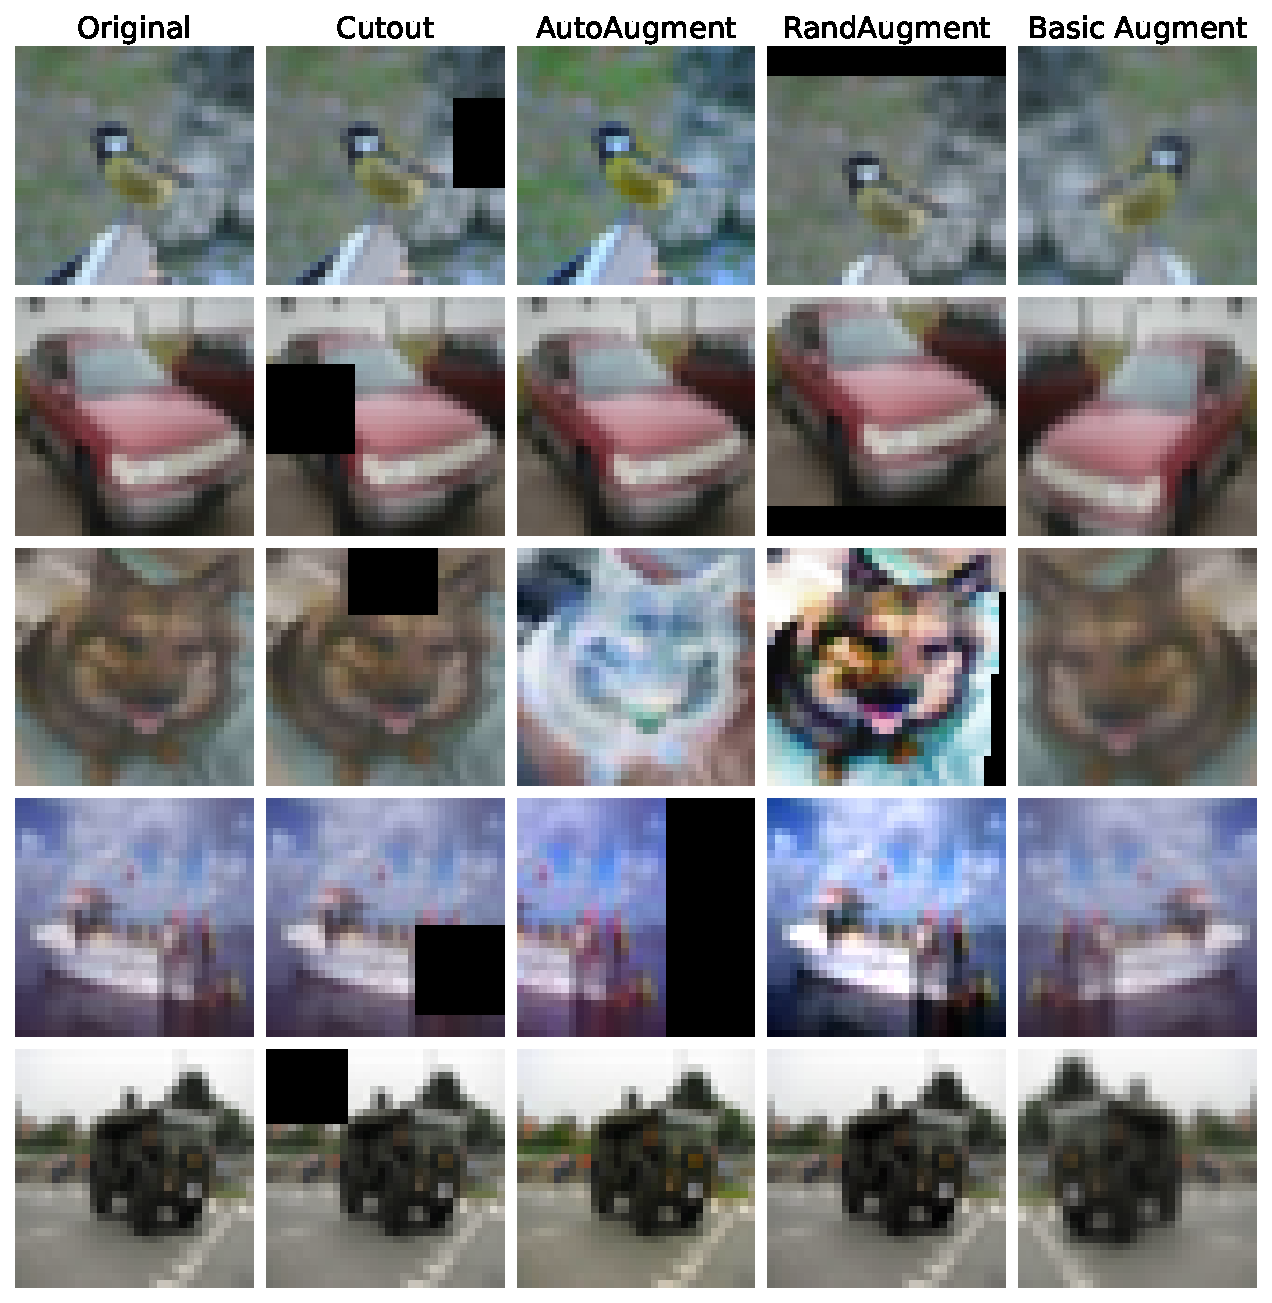
\includegraphics[width=\columnwidth]{augmentation_examples.pdf}
    \caption{Examples of data augmentation on a CIFAR-10. From left to right: Original, Cutout, AutoAugment, RandAugment, basic Augment (Crop, Flip).}
    \label{fig:example-data-aug}
\end{figure}

This lightweight augmentation pipeline provides a scalable and effective solution for addressing class imbalance, making it particularly valuable in real-world applications where data distributions are naturally skewed, such as medical diagnosis, fraud detection, and rare event prediction. By integrating efficient augmentation strategies, this approach improves fairness, accuracy, and generalization in classification models while maintaining a practical balance between performance and computational cost.

% \begin{algorithm}[htb]
% \SetAlgoLined
% \textbf{Required:} Dataset $D = \{(\mathbf{x}_i, y_i)\}_{i=1}^n$, model with parameter $\theta$\;
% \textbf{Hyperparameters:} $\alpha$, $\gamma$, batch size $M$, learning rate $\delta$, $\beta$ for \textit{effective number}\;
% Compute number of samples $n_c$ for each class $c$\;
% Compute class weight $w_c = \frac{1 - \beta}{1 - \beta^{n_c}}$ for each class\;
% Normalize weight: $w_c \gets \frac{w_c}{\sum_k w_k}$\;
% Initialize model parameter $\theta$\;
% \While{training}{
%   Sample batch $\{(\mathbf{x}_i, y_i), (\mathbf{x}_j, y_j)\}_{m=1}^M$ from $D$ using WeightedRandomBatchSampler or WeightedFixedBatchSampler with $\alpha$\;
%   Sample $\lambda_x \sim \mathit{Beta}(\gamma, \gamma)$\;
%   \For{$m = 1$ to $M$}{
%     (a) Obtain mixed input: $\tilde{\mathbf{x}}_m = \lambda_\mathbf{x} \mathbf{x}_i + (1 - \lambda_\mathbf{x}) \mathbf{x}_j$\;
%     (b) Compute label mixing coefficient $\lambda_y = \lambda_x$ or re-compute based on logits margin\;
%     (c) Mix label: $\tilde{y}_m = \lambda_y y_i + (1 - \lambda_y) y_j$\;
%   }
%   Compute loss: $\mathcal{L}(\theta) = \frac{1}{M} \sum_{m=1}^{M} w_{\tilde{y}_m} \cdot L(f(\tilde{\mathbf{x}}_m), \tilde{y}_m)$\;
%   Update parameters: $\theta \gets \theta - \delta \nabla_\theta \mathcal{L}(\theta)$\;
% }
% % \caption{Light-weight data augmentation framework training algorithm.}
% \end{algorithm}

\begin{algorithm}[htb]
\SetAlgoLined

\textbf{Required:} Dataset $D = \{(\mathbf{x}_i, y_i)\}_{i=1}^n$, model with parameter $\theta$\;
\textbf{Hyperparameters:} $\alpha$, $\gamma$, batch size $M$, learning rate $\delta$, $\beta$ for \textit{effective number}\;

Compute number of samples $n_c$ for each class $c$\;
Compute class weight $w_c = \frac{1 - \beta}{1 - \beta^{n_c}}$ for each class\;
Normalize weight: $w_c \gets \frac{w_c}{\sum_k w_k}$\;
Initialize model parameter $\theta$\;

\While{training}{
  Sample batch $\{(\mathbf{x}_i, y_i),(\mathbf{x}_j, y_j)\}_{m=1}^M$ from $D$ using 
  \texttt{WeightedRandomBatchSampler} or \texttt{WeightedFixedBatchSampler} with $\alpha$\;

  Sample $\lambda_x \sim \mathrm{Beta}(\gamma,\gamma)$\;

  \For{$m = 1$ to $M$}{
    Obtain mixed input:
    $\tilde{\mathbf{x}}_m = \lambda_x \mathbf{x}_i + (1-\lambda_x)\mathbf{x}_j$\;

    Compute label mixing coefficient $\lambda_y = \lambda_x$, or re-compute based on logits margin\;

    Mix label:
    $\tilde{y}_m = \lambda_y y_i + (1-\lambda_y)y_j$\;
  }

  Compute loss:
  $\mathcal{L}(\theta) =
  \frac{1}{M}\sum_{m=1}^{M}
  w_{\tilde{y}_m}
  L\bigl(f(\tilde{\mathbf{x}}_m),\tilde{y}_m\bigr)$\;

  Update parameters:
  $\theta \gets \theta - \delta \nabla_\theta \mathcal{L}(\theta)$\;
}

\caption{Light-weight data augmentation framework training algorithm.}
\label{alg:lightweight-augmentation}
\end{algorithm}

The effectiveness of the proposed approaches lies in their ability to balance computational efficiency and discriminative feature representation. Unlike naive resampling methods that may distort the intrinsic data distribution, these training strategies—particularly re-weighting and mixup-based augmentation—offer robust alternatives by leveraging class-balanced weighting and convex sample interpolation. While such methods enhance generalization under class imbalance, they also require careful tuning of hyperparameters (\textit{e.g., mixup intensity, weighting schedule}) to avoid label noise and maintain semantic consistency across classes.

\vspace{0.5em}
\noindent
The standard cross-entropy loss for a model output $\mathbf{z}_i \in \mathbb{R}^C$ (\textit{the logits}) and a target class $c \in \{1, \dots, C\}$ is defined as:
{\footnotesize
\begin{equation}
\mathcal{L}_{\mathrm{CE}}
= -\frac{1}{N} \sum_{i=1}^{N}
    \log \frac{\exp(z_{i, c})}{\sum_{j=1}^{C} \exp(z_{i, j})}
= -\frac{1}{N} \sum_{i=1}^{N}
    \log \big( \phi(\mathbf{z}_i)_{c} \big),
\end{equation}}
where $\phi(\cdot)$ denotes the softmax mapping from logits to class probabilities.

% ---------------------------------------------------------------------
\subsection{Empirical Risk Minimization (ERM)}
ERM treats all training samples equally without considering label imbalance. This serves as the baseline for comparison against adaptive re-weighting or augmentation strategies.

% ---------------------------------------------------------------------
\subsection{Deferred Re-Weighting (DRW):}
DRW mitigates imbalance by assigning class-dependent weight that evolve over training epochs.  
For each class $c$, a weight inversely proportional to its effective number of samples is defined as equation (3) and (4).
Weight is normalized to maintain comparability across classes:
\begin{equation}
w_c \leftarrow \frac{C w_c}{\sum_{j=1}^{C} w_j}.
\end{equation}
The weighted cross-entropy loss becomes:
\begin{equation}
\mathcal{L}_{\mathrm{DRW}}
= -\frac{1}{N} \sum_{i=1}^{N}
    w_{c} \log \big( \phi(\mathbf{z}_i)_{c} \big).
\end{equation}
By gradually activating class weight during training, DRW enables stable feature learning in early epochs and better balance in later stages.

% ---------------------------------------------------------------------
\subsection{Mixup:}
Mixup enhances generalization by linearly interpolating samples and labels such as Eq. \eqref{mixup_x} and 
Eq. \eqref{mixup_y} from section \ref{Mixup_interpolation}.
The loss is a convex combination of cross-entropies:
\begin{equation}
\mathcal{L}_{\mathrm{Mixup}}
= \lambda \, \mathcal{L}_{\mathrm{CE}}(\mathbf{z}, y_i)
+ (1 - \lambda) \, \mathcal{L}_{\mathrm{CE}}(\mathbf{z}, y_j),
\end{equation}
where $\mathbf{z}$ is the model output for the mixed input $\tilde{\mathbf{x}}$.  
Mixup smooths class boundaries and reduces overfitting by enforcing locally linear decision regions.

% ---------------------------------------------------------------------
\subsection{Imbalanced Lightweight Hybrid (ILWH) Loss:}
The ILWH objective integrates the Mixup formulation from Eq. \eqref{mixup_x} and 
Eq. \eqref{mixup_y} with the DRW scheme to achieve both data interpolation and adaptive class balancing.

\paragraph{Deferred class weight.}
Let $n_c$ denote the number of samples in class $c$. The normalized class weight is defined as:
\begin{equation}
w_c(\beta) = \frac{1 - \beta}{1 - \beta^{n_c}}, \qquad
\hat{w}_c(\beta) = \frac{C \, w_c(\beta)}{\sum_{k=1}^{C} w_k(\beta)}.
\end{equation}

\paragraph{ILWH loss}
Given the mixed samples $(\tilde{\mathbf{x}}, \tilde{\mathbf{y}})$ obtained as previously described and the corresponding model outputs $\mathbf{z}_i$, the overall batch objective is:
\begin{align}
&\mathcal{L}_{\mathrm{ILWH}}
= \frac{1}{N} \sum_{i=1}^{N}
\Big[
    \lambda \, \hat{w}_{c}(\beta) \,
        \big(-\log \phi(\mathbf{z}_i)_{y_i}\big) \nonumber \\ 
        &\quad \quad \quad \quad + (1 - \lambda) \,
        \hat{w}_{c}(\beta) \,
        \big(-\log \phi(\mathbf{z}_i)_{y_j}\big)
\Big], \\
&=\lambda \, \hat{w}_{c}(\beta) \,\mathcal{L}_{\mathrm{CE}}(\mathbf{z}, y_i) + (1 - \lambda) \, \hat{w}_{c}(\beta) \,\mathcal{L}_{\mathrm{CE}}(\mathbf{z}, y_j).
\end{align}

where $\lambda \sim \mathrm{Beta}(\gamma, \gamma)$ controls the interpolation strength, 
and $\mathcal{L}_{\mathrm{CE}}(\mathbf{z}, y_i)$ denotes the cross-entropy loss 
between the model output $\mathbf{z}$ and target label $y_i$.  

\vspace{0.5em}
\noindent
In all cases, the softmax operator $\phi(\cdot)$ transforms logits into class probabilities:
\begin{equation}
\phi(\mathbf{z})_c = \frac{\exp(z_c)}{\sum_{j=1}^{C} \exp(z_j)}.
\end{equation}

Moreover, we are also conducting further investigations to determine the optimal timing and conditions to apply augmentation techniques. Understanding\textit{ when and how} to introduce data augmentation is crucial, as different augmentation strategies may yield varying levels of effectiveness depending on the dataset characteristics, model architecture, and training dynamics. Our objective is to identify the most suitable augmentation approach for each specific method, ensuring that augmentation is neither underutilized nor excessively applied in ways that might introduce noise or degrade model performance. By systematically analyzing augmentation placement within the training pipeline, we aim to develop a \textit{more adaptive and context-aware augmentation strategy}, enabling better generalization and performance across diverse machine learning applications.

\subsection{Data Augmentation Approach}
We investigate the effectiveness of lightweight data augmentation methods: \textit{Cutout}, \textit{AutoAugment} and \textit{RandAugment}, for enhancing model generalization in the context of imbalance learning. These methods are selected due to their proven performance in previous studies, ease of implementation, and computational efficiency. An example of the effect of these techniques is shown in \ref{fig:example-data-aug}.

\subsubsection{AutoAugment}
AutoAugment~\cite{cubuk2018autoaugment} automatically searches for optimal augmentation policies to improve the validation accuracy of neural networks. Each augmentation policy comprises several sub-policies, each consisting of two sequential augmentation operations drawn from a predefined set. Specifically, a sub-policy \(S\) is defined by two augmentation operations (e.g., \textit{Shear, Rotate, Invert}): A probability associated with applying each operation and a magnitude indicating the strength of each operation.

AutoAugment formulates the search for optimal policies as a discrete optimization problem. Specifically, a controller, implemented as a recurrent neural network, samples augmentation sub-policies to form augmentation strategies. A child neural network is trained using these sampled policies and evaluated on a validation set. Validation accuracy serves as a reward signal that guides the search for policies using reinforcement learning, also known as policy gradient methods. Remarkably, AutoAugment has achieved state-of-the-art performance on datasets such as SVHN-10, CIFAR-10, CINIC-10, CIFAR-100, and TinyImageNet-200.
% \ha{the following sentence seems to be disconnected to the paragraph above. Linguistically, learned policies => not understandable}
% Although the search can be computationally expensive, learned policies have shown strong transferability between datasets, reducing the overall computational demand in practice.

\subsubsection{RandAug}
RandAugment~\cite{cubuk2019randaugment} addresses the computational complexity associated with AutoAugment by drastically reducing the augmentation search space and eliminating the separate proxy task. It uniformly applies random augmentation transformations with just two interpretable hyperparameters:
\begin{itemize}
    \item $N$: the number of augmentation operations applied sequentially.
    \item $M$: the global magnitude applied uniformly across transformations.
\end{itemize}

RandAugment randomly selects $N$ transformations from a predefined set (\textit{e.g., Rotate, TranslateX, Solarize, Color}), applying them sequentially at magnitude $M$. The simplified search space significantly reduces computational complexity from more than $10^{32}$ possibilities in AutoAugment to only $10^2$ possibilities, enabling straightforward grid searches for hyperparameter optimization~\cite{cubuk2019randaugment}.

RandAugment achieves competitive or superior performance compared to AutoAugment on standard benchmarks such as SVHN-10, CIFAR-10, CINIC-10, CIFAR-100, and TinyImageNet-200 while drastically reducing the computational resources required.

\subsubsection{Cutout}
\label{subsec:cutout}
\textit{Cutout} is a lightweight regularization method where a contiguous rectangular patch is removed (\textit{i.e., zeroed out}) from each training image at a random location~\cite{devries2017cutout}. This procedure generates partially occluded samples that effectively expand the diversity of the training set. Unlike typical dropout variants, \textit{Cutout} is applied directly to the input image rather than intermediate features. As a result, downstream feature maps corresponding to the masked region are forced to focus on contextual information surrounding the missing patch, helping the model rely on broader cues in the data~\cite{devries2017cutout}.

Suppose each training image has spatial dimensions of H$\times$ W. \textit{Cutout} selects a random center pixel \((c_x, c_y)\) within the image and replaces all pixels in a square patch of side length \(M\) (\textit{the primary hyperparameter of Cutout}) with zeros. Parts of the square lying outside the image boundaries are simply discarded. For best performance, it is recommended to first normalize the image about zero to minimize distributional shifts introduced by zero-pixels. Furthermore, the value of \(M\) is typically empirically validated depending on the resolution and complexity of the dataset~\cite{devries2017cutout}.

% Cutout offers three key benefits. First, by simulating occluded objects, it encourages the network to learn from less discriminative regions and thus become more robust to real-world occlusions. Second, it can be easily combined with common data augmentation techniques such as flipping or cropping, as well as methods like AutoAugment or RandAugment~\cite{cubuk2018autoaugment, cubuk2019randaugment}. Finally, it is straightforward to implement, typically requiring only a few lines of code during data loading.


\subsection{Data Sampling Approach}

To establish a baseline for analyzing the effectiveness of batch sampling approaches, we implemented a standard Empirical Risk Minimization (ERM) strategy without any batch sampling interventions. This baseline provides a comparison point for assessing the impact of different sampling methods. The model was trained on an imbalanced dataset, and performance metrics such as accuracy, precision, and F1-score were recorded. The results highlighted the challenges of training on imbalanced datasets, where minority class accuracy and generalization were significantly lower than those of majority classes.

We conducted two primary batch sampling methods to address the imbalance in class distributions:

\begin{itemize}
    \item \textit{Weighted Random Batch Sampler (WRBS)} This method samples with replacement based on dynamically computed weight for each class. It probabilistically selects samples according to their assigned weight, ensuring diversity in class representation within each batch, but allowing variability in batch composition across training epochs.

    \item \textit{Weighted Fixed Batch Sampler (WFBS)} This method enforces strict proportions of samples per class in each batch. By ensuring a fixed number of samples from each class, WFBS maintains consistent class representation across batches, which is critical for scenarios requiring precise balancing.
\end{itemize}
% put this macro in your preamble

\paragraph{Alpha Parameter $\alpha$} Both samplers incorporate an adjustable parameter $\alpha$ to balance between:
\begin{itemize}
    \item \textit{Training population class distribution:} The weight is proportional to the original class sizes in the dataset.
    \item \textit{Uniform distribution:} All classes are equally represented.
\end{itemize}

The combined weight \( w_i \) for each class is computed as:
\begin{equation}
w_i = \alpha \cdot w_i^{u} + (1 - \alpha) \cdot w_i^{o},
\end{equation}
where: $w_i^{u} = \frac{1}{C}$: \text{uniform weight}, $w_i^{o} = \frac{n_i}{N}$: \text{original weight}, and $\alpha \in [0, 1]$.
Here, \(C\) is the total number of classes, \(n_i\) is the number of samples in class \(i\), and \(N\) is the total number of samples in the dataset. \(\alpha = 0\) relies entirely on the original class distribution, while \(\alpha = 1\) creates a uniform distribution. Intermediate values of \(\alpha\) strike a balance between the two.

% \ha{What is difference between eq 3 and eq 6? - \textbf{Duy}: duplicated content - will remove one of 2}

\paragraph{Hypothesis from Baseline}
The baseline results demonstrated severe bias towards the majority classes, leading to suboptimal performance on minority classes. Based on this, our hypothesis is as follows:
\begin{itemize}
    \item Implementing \textit{Weighted Random Batch Sampler (WRBS)} will improve minority class accuracy due to its adaptive sampling strategy, but the variability in batch composition may cause fluctuations during training.
    \item Using \textit{Weighted Fixed Batch Sampler (WFBS)} will offer consistent improvement in class representation across batches, leading to more stable training and better generalization compared to WRBS.
    \item Increasing \(\alpha\) (\textit{i.e., moving towards a uniform distribution}) will enhance generalization by ensuring fair representation of minority classes but may reduce model focus on majority classes, impacting overall accuracy.
\end{itemize}

\newcommand{\valpm}[2]{%
  \ensuremath{#1\,{\scriptstyle\pm}\,#2}%
}

\begin{table*}[t]
\centering
\caption{Average top-1 validation accuracy (\%, mean $\pm$ std) of different sampling methods with different sampling parameters and  with imbalance ratio 0.01. Best results are highlighted in \textbf{bold}. \label{tab:merged_comparison}}
\setlength{\tabcolsep}{5pt}
\begin{tabular}{l c cc cc cc}
\toprule
\toprule
\multirow{2}{*}{\textbf{Sampling Method}} & \multirow{2}{*}{$\alpha$} 
& \multicolumn{2}{c}{\textbf{CIFAR-10}} 
& \multicolumn{2}{c}{\textbf{SVHN-10}} 
& \multicolumn{2}{c}{\textbf{CIFAR-100}} \\
\cmidrule(lr){3-4} \cmidrule(lr){5-6} \cmidrule(lr){7-8}
& & ERM & ILWH (Ours) & ERM & ILWH (Ours) & ERM & ILWH (Ours) \\
\midrule
\midrule
\multirow{3}{*}{\textbf{WRBS}}
 & $\alpha=0.5$ & \valpm{71.76}{0.24} & \valpm{81.66}{0.42} & \textbf{\valpm{82.79}{0.29}} & \valpm{81.69}{0.16} & \valpm{38.59}{0.22} & \textbf{\valpm{47.82}{0.38}} \\
 & $\alpha=0.7$ & \valpm{71.97}{0.61} & \valpm{81.74}{0.17} & \valpm{81.44}{0.18} & \valpm{81.46}{0.42} & \valpm{37.56}{0.24} & \valpm{46.15}{0.41} \\
 & $\alpha=1.0$ & \valpm{71.65}{0.62} & \textbf{\valpm{82.41}{0.21}} & \valpm{82.79}{0.25} & \valpm{81.20}{0.36} & \valpm{35.34}{0.58} & \valpm{44.88}{0.52} \\
\midrule
\multirow{3}{*}{\textbf{WFBS}}
 & $\alpha=0.5$ & \valpm{71.93}{0.61} & \valpm{82.09}{0.38} & \valpm{80.56}{0.17} & \valpm{82.00}{0.31} & \valpm{37.12}{0.26} & \textbf{\valpm{45.79}{0.35}} \\
 & $\alpha=0.7$ & \valpm{71.61}{0.64} & \textbf{\valpm{82.20}{0.18}} & \valpm{81.16}{0.57} & \valpm{81.52}{0.32} & \valpm{36.48}{0.30} & \valpm{44.93}{0.42} \\
 & $\alpha=1.0$ & \valpm{71.95}{0.65} & \valpm{81.95}{0.23} & \valpm{80.95}{0.18} & \textbf{\valpm{82.56}{0.25}} & \valpm{34.85}{0.61} & \valpm{43.71}{0.47} \\
\midrule
\textbf{Random \cite{cheng2023smote}} 
 & -- & \valpm{71.23}{0.51} & \valpm{82.11}{0.57} & \valpm{79.97}{0.67} & \valpm{85.19}{0.32} & \valpm{38.46}{0.36} & \valpm{46.91}{0.46} \\
\bottomrule
\bottomrule
\end{tabular}
\end{table*}
\section{Ablation Study} \label{sec:ablation}
% \subsection{Impact of the Sampling Hyperparameter \(\alpha\)}

To understand the influence of our sampling strategies, we conducted an ablation study on the hyperparameter \(\alpha\), which controls the degree of class balancing in our samplers. The parameter \(\alpha\) interpolates between the original data distribution (\(\alpha=0\)) and a perfectly uniform class distribution (\(\alpha=1\)). A higher value of \(\alpha\) enforces more aggressive rebalancing by increasing the sampling rate of minority classes. The results of this analysis across three datasets are presented in Table~\ref{tab:merged_comparison}. 

On CIFAR-10, a higher degree of balancing generally proves beneficial when using the advanced \textbf{I}mbalanced \textbf{L}ight\textbf{W}eight \textbf{H}ybrid (ILWH) training scheme. For WRBS, performance peaks at \(\alpha=1.0\) (82.41\%), while for WFBS, the sweet spot is at \(\alpha=0.7\) (82.20\%). This indicates that for this 10-class problem, aggressively rebalancing the dataset allows the model to better learn minority class features without significantly degrading performance on majority classes.

In contrast, on the more complex CIFAR-100 dataset, a less aggressive balancing strategy (\(\alpha=0.5\)) consistently yields the best results for both WRBS (47.82\%) and WFBS (45.79\%) under the ILWH setting. Performance for both samplers degrades as \(\alpha\) increases toward 1.0. This suggests that in a fine-grained classification scenario with many classes, overly aggressive sampling of the rare classes can cause the model to under-learn the diverse features present in the more populated ``head'' classes, ultimately harming overall accuracy.

The results on SVHN-10 present another interesting case. Here, the standard \textbf{Random} sampling, when paired with ILWH, achieves the highest accuracy (85.19\%), outperforming all tuned \(\alpha\) values for both WRBS and WFBS. This suggests that for certain datasets, the powerful regularization provided by the training method ILWH may be more impactful than the specific batch-level balancing strategy, making aggressive re-sampling less critical or even slightly detrimental.

In conclusion, the choice of \(\alpha\) is not one-size-fits-all. While stronger balancing can be effective, it carries the risk of model underfitting on majority classes. Our results suggest using a conservative value like \(\alpha=0.5\) as a strong starting point, especially for complex datasets with many classes, and treating it as a key hyperparameter to be tuned based on the specific characteristics of the task at hand.
% \paragraph{AutoAugment}
% AutoAugment introduces a learned sequence of augmentation policies, which diversifies the training data by applying a complex set of transformations discovered through a search process. During training, the exposure of the network to such a wide array of augmented samples aims to enhance model robustness by preventing it from overfitting to the original, potentially limited, training instances. The subsequent normalization of these augmented images, based on the dataset's statistical properties, is anticipated to stabilize the training trajectory and potentially accelerate convergence by standardizing the input distribution presented to the network. The core impact on training is the broadened feature space exploration, compelling the model to learn more generalizable representations.

% \paragraph{RandAugment}
% RandAugment simplifies the automated augmentation paradigm by applying a randomly selected sequence of $N$ transformations, each with a global magnitude $M$. This approach introduces a controlled yet stochastic element to the training data pipeline. The random application of these transformations acts as a dynamic regularizer, potentially smoothing the loss landscape and guiding the model towards flatter minima, which are often associated with better generalization. By varying $N$ and $M$, the intensity of augmentation can be tuned, directly influencing the degree of perturbation in the training samples and thereby affecting the model's sensitivity to input variations learned during training. The primary effect on training is the consistent introduction of novel data variations with minimal computational overhead compared to more complex search-based methods.

% \paragraph{Cutout}
% Cutout operates by randomly excising square regions from input images during training. This technique imposes a unique form of spatial regularization, compelling the network to learn from a more comprehensive set of contextual cues within an image, rather than focusing on a few dominant, localized features. By simulating occlusions, Cutout encourages the model to develop more robust and distributed feature representations during the training phase. This can be particularly beneficial in preventing the model from becoming overly reliant on specific visual patterns that might be prevalent in the majority classes or distinctive but not generalizable features of minority classes. Its application during data loading introduces minimal computational burden, making it an efficient method to enhance feature learning throughout the training epochs.



% \section{Potential Lightweight Approaches in Imbalanced Classification}

% The ablation study systematically evaluates the incremental contributions of each component within the proposed lightweight augmentation and sampling pipeline. By sequentially adding components and carefully analyzing their impacts, we uncover the effectiveness, limitations, and interplay among various methods designed to handle imbalanced data learning tasks.

% \paragraph{Impact of Lightweight Data Augmentation}
% To quantify the benefits of lightweight data augmentation methods, we evaluate three widely-used augmentation techniques: Cutout, AutoAugment, and RandAugment. Applying Cutout—randomly masking regions of input images—provides modest improvement by forcing the model to consider broader contextual features. However, this technique sometimes inadvertently masks critical features for minority classes, thus reducing its potential impact in scenarios with severe class imbalance. Subsequently, AutoAugment, which leverages reinforcement learning to automatically determine optimal augmentation policies, shows notable improvement. Its strength lies in its adaptability, discovering augmentation strategies suited specifically for the CIFAR-10 dataset. However, AutoAugment incurs considerable computational costs due to its policy search phase, limiting practical deployment, especially in resource-constrained environments. RandAugment simplifies this search by applying randomly selected transformations with adjustable intensity parameters. Our results indicate RandAugment consistently achieves superior or comparable performance compared to AutoAugment, but with significantly reduced computational overhead. This highlights RandAugment as a particularly suitable choice when balancing computational efficiency and performance improvements.

% % To further strengthen the insights provided here, an additional experiment evaluating computational resource usage (e.g., training time and memory consumption) explicitly comparing RandAugment and AutoAugment would be beneficial. A graphical illustration highlighting computational cost versus performance gains would provide valuable empirical evidence for recommending RandAugment in practice.

% \paragraph{Integration of Mixup and DRW}
% The integration of Mixup augmentation with Deferred Re-weighting (DRW) significantly enhances model performance. Mixup interpolates between pairs of training samples, thereby softening decision boundaries and improving generalization across imbalanced classes. DRW dynamically adjusts class weights during training, ensuring minority classes receive appropriate emphasis as training progresses. Our results confirm that combining Mixup with DRW consistently improves classification accuracy across all sampling strategies evaluated. Nonetheless, the performance depends heavily on careful tuning of Mixup parameters (such as the mixing parameter $\alpha$). Incorrect parameterization may introduce excessive noise, especially in minority classes, negatively affecting model generalization. To strengthen this finding, conducting experiments analyzing the sensitivity of model performance to the Mixup hyperparameter $\alpha$ would provide valuable insights. Visualization of model accuracy and loss curves as a function of $\alpha$ would clearly illustrate optimal operational ranges, enhancing both theoretical insights and practical guidelines.

% \paragraph{Analysis of Sampling Strategies}
% Next, we assess two sampling techniques: WeightedRandomBatchSampler (WRBS) and WeightedFixedBatchSampler (WFBS). WRBS dynamically samples data based on class-specific weights, ensuring diverse class representations within each batch. Experimental results confirm WRBS effectively improves minority class accuracy by providing richer exposure to underrepresented samples during training. However, WRBS-induced variability in batch compositions across epochs may cause fluctuations in training stability and potentially affect convergence. Conversely, WFBS enforces strict, fixed class proportions per batch, ensuring stable and consistent batch compositions. While WFBS generally improves minority-class generalization due to consistency, its rigid structure makes it less adaptable to datasets with evolving distributions. Consequently, WFBS may limit performance improvements when class distributions dynamically shift during training or across datasets. A comparative analysis between these two sampling methods using additional datasets with differing class-imbalance characteristics would substantially enhance generalization of these findings. Additionally, visualizations of training dynamics (such as accuracy, precision, and loss convergence graphs) under WRBS versus WFBS would clarify their respective strengths and weaknesses, assisting practitioners in selecting the optimal sampling method for their specific use-case.

% \paragraph{DRW}

\begin{figure}[htb]
    \centering
    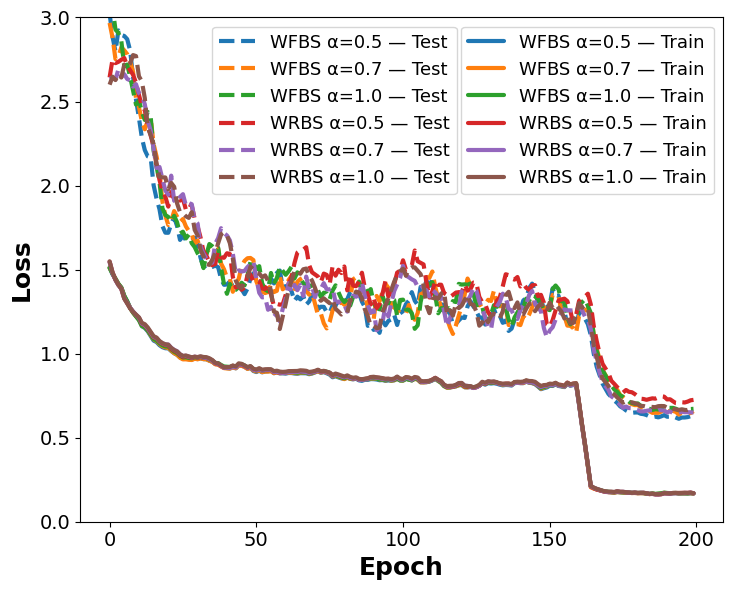
\includegraphics[width=0.9\columnwidth]{drw_affect.png}
        \caption{Effect of applying DRW. After the $160^{th}$ epoch, we apply DRW and observe that the losses have significantly decreased.}
\label{fig:drw_affect}
\end{figure}
\begin{figure}[htb]
    \centering
    \begin{subfigure}[b]{0.48\columnwidth}
        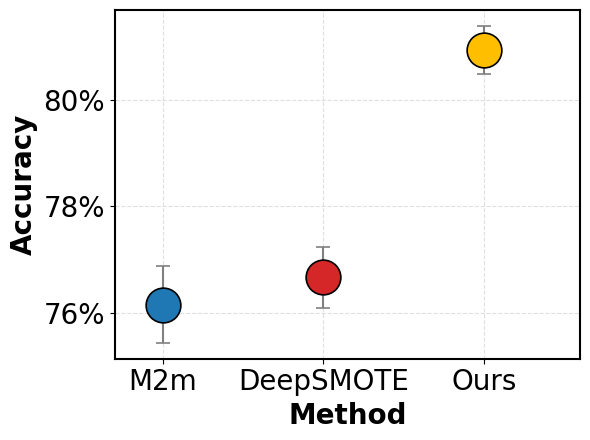
\includegraphics[width=\columnwidth]{cifar10_comparision.png}
        \caption{CIFAR-10}
        % \vspace{-7pt}
        \label{fig:cifar10_comparisionA}
    \end{subfigure}
    \begin{subfigure}[b]{0.48\columnwidth}
        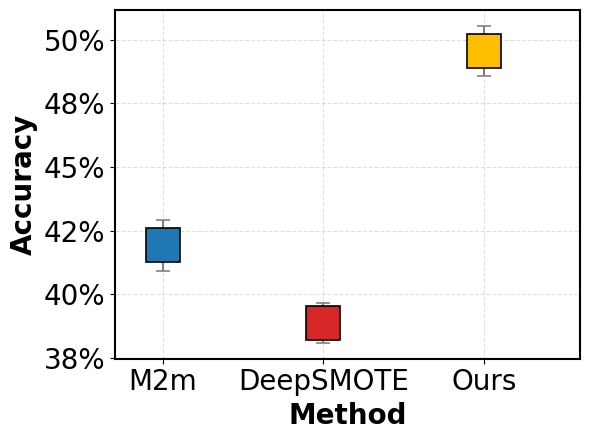
\includegraphics[width=\columnwidth]{cifar100_comparision.png}
        \caption{CIFAR-100}
        % \vspace{-7pt}
        \label{fig:cifar100_comparisionB}
    \end{subfigure}
    \caption{The comparison of our lightweight method and the other resource-intensive methods model performance on CIFAR-10 and CIFAR-100 dataset. This result (M2m, DeepSMOTE \cite{cheng2023smote} and Ours)  demonstrates that our method archive competitive performance.}   \label{fig:comparision_m2m_deepSMOTE_Ours}
\end{figure}
\begin{figure}
    \centering
    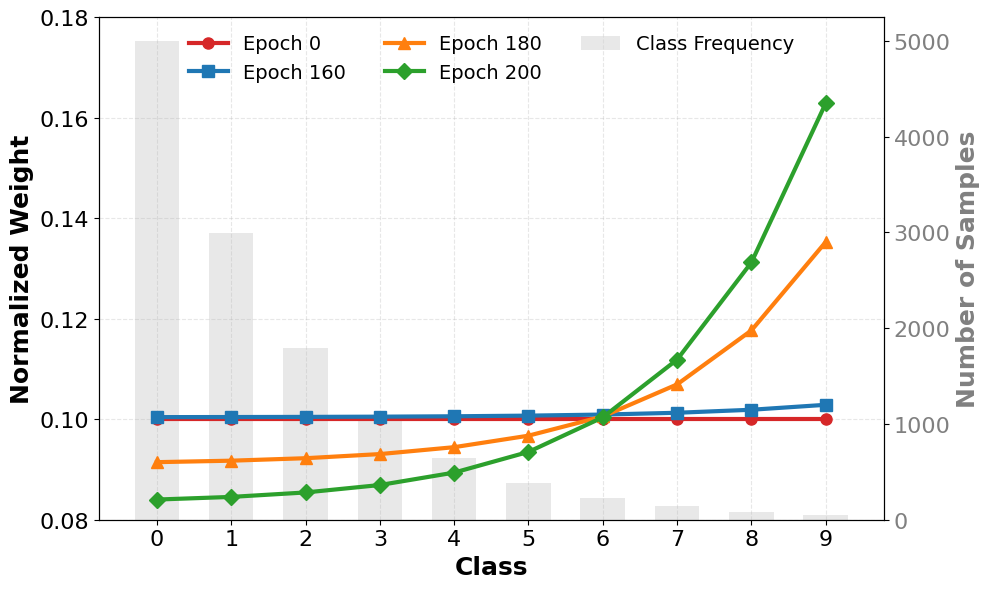
\includegraphics[width=\columnwidth]{weight_dist.png}
        % \vspace{-7pt}
    \caption{Weight distribution for CIFAR-10 classes before and after applying DRW.}
    \label{fig:weight_dist}
\end{figure}

% \begin{table*}[t]
% \centering
% \caption{Performance comparison of different sampling methods and augmentations across CIFAR-10, SVHN-10, and CINIC-10 datasets. \label{tab:drw_results_cifar_svhn_cinic}}
% \scalebox{0.68}{
% \begin{tabular}{l|c| cccc | cccc | cccc }
% \toprule
% \toprule
% \multirow{2}{*}{Sampling} & \multirow{2}{*}{Augmentation} 
%     & \multicolumn{4}{c}{\textbf{CIFAR-10}} 
%     & \multicolumn{4}{c}{\textbf{SVHN-10}} 
%     & \multicolumn{4}{c}{\textbf{CINIC-10}} \\
% \cmidrule(lr){3-6} \cmidrule(lr){7-10} \cmidrule(lr){11-14}
% & & ERM & DRW & Mixup & ILWH (Ours) 
%   & ERM & DRW & Mixup & ILWH (Ours) 
%   & ERM & DRW & Mixup & ILWH (Ours) \\
% \midrule
% \midrule
% \multirow{4}{*}{\textbf{Random}} 
%     & Baseline & 72.74\scriptsize{$\pm$0.42} & 76.03\scriptsize{$\pm$0.05} &   73.37\scriptsize{$\pm$0.15} & \textbf{82.19\scriptsize{$\pm$0.17}} 
%                 & 81.60$\pm$0.28 & 80.57$\pm$0.79 & 80.73$\pm$0.43 & 85.52$\pm$0.26 
%                 & 60.65$\pm$0.39 & 64.29$\pm$0.22 &  63.75$\pm$0.57 & 71.21$\pm$0.19 \\
%     % \cmidrule(lr){2-14}
%     & Cutout   & 72.15$\pm$0.48 & 75.65$\pm$0.39 & 73.32$\pm$0.66 & 81.84$\pm$0.12 
%                 & 85.40$\pm$0.63 & 86.78$\pm$0.30 &  81.53$\pm$0.78  & 86.32$\pm$0.11 
%                 & 64.52$\pm$0.42  & 68.55$\pm$0.32 &  65.70$\pm$0.68 & 73.55$\pm$0.16 \\
%     % \cmidrule(lr){2-14}
%     & AutoAug  & 75.15 $\pm$ 0.35 & 79.08 $\pm$ 0.46 & 72.96 $\pm$ 0.21   & 81.97 $\pm$ 0.13 
%                 & \textbf{85.78 $\pm$ 0.30} & \textbf{86.80 $\pm$ 0.83} & 85.86 $\pm$ 0.21   & \textbf{88.20 $\pm$ 0.49} 
%                 & 63.83 $\pm$ 0.20 & 68.99 $\pm$ 0.50 &  65.35  $\pm$ 0.32    & 73.36 $\pm$ 0.29  \\
%     % \cmidrule(lr){2-14}
%     & RandAug  & \textbf{75.72 $\pm$ 0.38} & \textbf{80.94 $\pm$ 0.12} &   73.77 $\pm$ 0.26 & 81.36 $\pm$ 0.61 
%                 & 84.62 $\pm$ 0.43 & 85.58 $\pm$ 0.91 &  83.08 $\pm$ 0.65   & 86.82 $\pm$ 0.33 
%                 & 64.71 $\pm$ 0.06 & 70.52 $\pm$ 0.27  &  65.92 $\pm$ 0.46  & 73.61 $\pm$  0.16 \\
% \midrule
% \multirow{4}{*}{\textbf{WRBS}} 
%     & Baseline & -- & -- & -- & -- & -- & -- & -- & -- & 60.68 $\pm$ 0.45 & -- & -- & -- \\
%     % \cmidrule(lr){2-14}
%     & Cutout   & -- & -- & -- & -- & -- & -- & -- & -- &  64.34 $\pm$ 0.45  & -- & -- & -- \\
%     % \cmidrule(lr){2-14}
%     & AutoAug  & -- & -- & -- & -- & -- & -- & -- & -- & 63.81 $\pm$ 0.51  & -- & -- & -- \\
%     % \cmidrule(lr){2-14}
%     & RandAug  & -- & -- & -- & -- & -- & -- & -- & -- & 65.16 $\pm$ 0.36 & -- & -- & -- \\
% \midrule
% \multirow{4}{*}{\textbf{WFBS}} 
%     & Baseline & 71.80 $\pm$ 0.60&   75.21 $\pm$ 0.65    &   73.36 $\pm$ 0.39  &  81.91  $\pm$ 0.33   & 80.41 $\pm$ 0.20 &   80.43 $\pm$ 0.83 &  81.14 $\pm$ 0.29  & 85.59 $\pm$ 0.44 & --  & -- & -- & -- \\
%     % \cmidrule(lr){2-14}
%     & Cutout   &  75.38 $\pm$ 0.46 & 79.90 $\pm$  0.79 &   73.49 $\pm$ 0.65 &   81.47 $\pm$ 0.17 & 84.01 $\pm$ 0.50 &   85.64 $\pm$ 1.04 &  82.49 $\pm$ 1.28 &  86.14 $\pm$ 0.59 &   -- &  --  & -- & -- \\
%     % \cmidrule(lr){2-14}
%     & AutoAug  & 74.23 $\pm$ 0.30 & 79.54 $\pm$  0.52 &  73.63 $\pm$ 0.86   & 82.00 $\pm$ 0.17  & 85.30 $\pm$  0.70 &  86.39 $\pm$ 0.64   &  85.05 $\pm$ 0.31 & 88.43 $\pm$ 0.56 & --  & -- & -- & -- \\
%     % \cmidrule(lr){2-14}
%     & RandAug  &  75.24 $\pm$  1.20  &  80.92 $\pm$ 0.24  &  74.03 $\pm$ 0.41 &  81.60 $\pm$ 0.21  & 83.92 $\pm$  1.71 &   84.85  $\pm$ 0.94 &   83.29 $\pm$ 0.78  &  87.46 $\pm$  0.41  & --  & -- & -- & -- \\
% \bottomrule
% \bottomrule
% \end{tabular}}
% \end{table*}

% In your preamble
% \newcommand{\valpm}[2]{#1{\tiny $\pm$#2}}
\begin{table*}[htb]
\centering
\caption{Performance comparison of different sampling methods and augmentations across CIFAR-10, SVHN-10, and CINIC-10 datasets with imbalance ratio 0.01. Best results are highlighted in \textbf{bold} while the runner up is \underline{\textit{underlined}}.}.
\label{tab:drw_results_cifar_svhn_cinic}
\renewcommand{\arraystretch}{1.5}
\setlength{\tabcolsep}{1.0pt}
\scalebox{0.80}{
\begin{tabular}{lc cccc cccc cccc }
\toprule
\toprule
\multirow{2}{*}{Sampling} & \multirow{2}{*}{Augmentation} 
    & \multicolumn{4}{c}{\textbf{CIFAR-10}} 
    & \multicolumn{4}{c}{\textbf{SVHN-10}} 
    & \multicolumn{4}{c}{\textbf{CINIC-10}} \\
\cmidrule(lr){3-6} \cmidrule(lr){7-10} \cmidrule(lr){11-14}
& & ERM & DRW & Mixup & ILWH (Ours) 
  & ERM & DRW & Mixup & ILWH (Ours) 
  & ERM & DRW & Mixup & ILWH (Ours) \\
\midrule
\midrule
\multirow{4}{*}{\textbf{Random}} 
    & Baseline & \valpm{72.74}{0.42} & \underline{\valpm{76.03}{0.05}} & \valpm{73.37}{0.15} & \textbf{\valpm{82.19}{0.17}} 
                & \underline{\valpm{81.60}{0.28}} & \valpm{80.57}{0.79} & \valpm{80.73}{0.43} & \textbf{\valpm{85.52}{0.26}} 
                & \valpm{60.65}{0.39} & \underline{\valpm{64.29}{0.22}} & \valpm{63.75}{0.57} & \textbf{\valpm{71.21}{0.19}} \\
    & Cutout   & \valpm{72.15}{0.48} & \underline{\valpm{75.65}{0.39}} & \valpm{73.32}{0.66} & \textbf{\valpm{81.84}{0.12}} 
                & \valpm{85.40}{0.63} & \textbf{\valpm{86.78}{0.30}} & \valpm{81.53}{0.78} & \underline{\valpm{86.32}{0.11}} 
                & \valpm{64.52}{0.42} & \underline{\valpm{68.55}{0.32}} & \valpm{65.70}{0.68} & \textbf{\valpm{73.55}{0.16}} \\
    & AutoAug  & \underline{\valpm{79.08}{0.46}} & \valpm{75.15}{0.35} & \valpm{72.96}{0.21} & \textbf{\valpm{81.97}{0.13}} 
                & \valpm{85.78}{0.30} & \underline{\valpm{86.80}{0.83}} & \valpm{85.86}{0.21} & \textbf{\valpm{88.20}{0.49}} 
                & \valpm{63.83}{0.20} & \underline{\valpm{68.99}{0.50}} & \valpm{65.35}{0.32} & \textbf{\valpm{73.36}{0.29}} \\
    & RandAug  & \underline{\valpm{80.94}{0.12}} & \valpm{75.72}{0.38} & \valpm{73.77}{0.26} & \textbf{\valpm{81.36}{0.61}} 
                & \valpm{84.62}{0.43} & \underline{\valpm{85.58}{0.91}} & \valpm{83.08}{0.65} & \textbf{\valpm{86.82}{0.33}} 
                & \valpm{64.71}{0.06} & \underline{\valpm{70.52}{0.27}} & \valpm{65.92}{0.46} & \textbf{\valpm{73.61}{0.16}} \\
\midrule
\multirow{4}{*}{\textbf{WRBS}} 
    & Baseline &  \valpm{71.14}{0.22} & \underline{\valpm{75.32}{0.42}} & \valpm{74.65}{0.10} & \textbf{\valpm{82.01}{0.46}} 
                & \underline{\valpm{82.96}{0.85}} & \valpm{81.07}{1.60} & \valpm{81.39}{0.62} & \textbf{\valpm{84.60}{2.02}} 
                & \valpm{60.68}{0.45} & \valpm{58.02}{1.80} & \underline{\valpm{62.42}{0.34}} & \textbf{\valpm{68.32}{0.17}} \\
    & Cutout   & \valpm{71.65}{1.21} & \underline{\valpm{75.46}{0.61}} & \valpm{73.46}{0.82} & \textbf{\valpm{81.30}{0.37}} 
                & \valpm{81.98}{1.43} & \underline{\valpm{84.49}{1.95}} & \valpm{83.20}{0.47} & \textbf{\valpm{85.33}{1.34}} 
                & \valpm{64.34}{0.45} & \valpm{61.74}{0.75} & \underline{\valpm{64.96}{0.74}} & \textbf{\valpm{69.07}{0.23}} \\
    & AutoAug  & \valpm{71.64}{0.06} & \underline{\valpm{75.31}{0.41}} & \valpm{73.77}{0.40} & \textbf{\valpm{82.35}{0.25}} 
                & \valpm{85.30}{0.70} & \underline{\valpm{86.39}{0.64}} & \valpm{86.07}{2.31} & \textbf{\valpm{88.43}{0.56}} 
                & \valpm{63.81}{0.51} & \valpm{61.48}{0.63} & \underline{\valpm{64.57}{0.42}} & \textbf{\valpm{69.61}{0.12}} \\
    & RandAug  & \valpm{71.52}{0.32} & \underline{\valpm{75.27}{0.21}} & \valpm{73.39}{0.11} & \textbf{\valpm{82.10}{0.44}} 
                & \valpm{85.17}{2.19} & \textbf{\valpm{87.45}{0.24}} & \valpm{87.35}{0.30} & \underline{\valpm{87.44}{0.42}} 
                & \valpm{65.16}{0.36} & \underline{\valpm{66.67}{0.38}} & \valpm{65.66}{0.35} & \textbf{\valpm{72.18}{0.39}} \\
\midrule
\multirow{4}{*}{\textbf{WFBS}} 
    & Baseline & \valpm{71.80}{0.60} & \underline{\valpm{75.21}{0.65}} & \valpm{73.36}{0.39} & \textbf{\valpm{81.91}{0.33}} 
                & \valpm{80.41}{0.20} & \valpm{80.43}{0.83} & \underline{\valpm{81.14}{0.29}} & \textbf{\valpm{85.59}{0.44}} 
                & \valpm{56.32}{0.90} & \valpm{60.62}{0.17} & \underline{\valpm{61.98}{0.27}} & \textbf{\valpm{69.43}{0.36}} \\
    & Cutout   & \underline{\valpm{79.90}{0.79}} & \valpm{75.38}{0.46} & \valpm{73.49}{0.65} & \textbf{\valpm{81.47}{0.17}} 
                & \valpm{84.01}{0.50} & \underline{\valpm{85.64}{1.04}} & \valpm{82.49}{1.28} & \textbf{\valpm{86.14}{0.59}} 
                & \valpm{56.74}{0.67} & \valpm{62.91}{0.35} & \underline{\valpm{63.31}{0.14}} & \textbf{\valpm{70.81}{0.21}} \\
    & AutoAug  & \underline{\valpm{79.54}{0.52}} & \valpm{74.23}{0.30} & \valpm{73.63}{0.86} & \textbf{\valpm{82.00}{0.17}} 
                & \valpm{85.30}{0.70} & \underline{\valpm{86.39}{0.64}} & \valpm{85.05}{0.31} & \textbf{\valpm{88.43}{0.56}} 
                & \valpm{61.47}{0.45} & \underline{\valpm{66.32}{0.12}} & \valpm{61.11}{0.28} & \textbf{\valpm{71.86}{0.16}} \\
    & RandAug  & \underline{\valpm{80.92}{0.24}} & \valpm{75.24}{1.20} & \valpm{74.03}{0.41} & \textbf{\valpm{81.60}{0.21}} 
                & \underline{\valpm{84.85}{0.94}} & \valpm{83.92}{1.71} & \valpm{83.29}{0.78} & \textbf{\valpm{87.46}{0.41}} 
                & \valpm{62.85}{0.55} & \underline{\valpm{66.31}{0.36}} & \valpm{66.02}{0.04} & \textbf{\valpm{71.68}{0.16}} \\
\bottomrule
\bottomrule
\end{tabular}}
\end{table*}
\begin{table*}[htb]
\centering
\caption{Performance comparison of different sampling methods and augmentations across CIFAR-100 and TinyImageNet-200 (TINY-200) datasets with imbalance ratio 0.01. Best results are highlighted in \textbf{bold} while the runner up is \underline{\textit{underlined}}.}
\label{tab:drw_results_cifar100_tiny}
\renewcommand{\arraystretch}{1.5}
\setlength{\tabcolsep}{3pt}
\scalebox{0.99}{
\begin{tabular}{lc cccc  cccc }
\toprule
\toprule
\multirow{2}{*}{Sampling} & \multirow{2}{*}{Augmentation} 
    & \multicolumn{4}{c}{\textbf{CIFAR-100}} 
    & \multicolumn{4}{c}{\textbf{TINY-200}} \\
\cmidrule(lr){3-6} \cmidrule(lr){7-10}
& & ERM & DRW & Mixup & ILWH (Ours) 
  & ERM & DRW & Mixup & ILWH (Ours) \\
\midrule
\midrule
\multirow{4}{*}{\textbf{Random}} 
    & Baseline & \valpm{38.87}{0.71} & \valpm{39.46}{0.50} & \underline{\valpm{41.57}{0.46}} & \textbf{\valpm{47.07}{0.47}} 
                & \underline{\valpm{34.17}{0.37}} & \valpm{33.90}{0.41} & \valpm{33.69}{0.29} & \textbf{\valpm{38.69}{0.10}} \\
    & Cutout   & \valpm{43.37}{0.05} & \underline{\valpm{46.12}{0.19}} & \valpm{42.02}{0.59} & \textbf{\valpm{49.56}{0.42}} 
                & \valpm{32.83}{0.36} & \valpm{31.64}{0.36} & \underline{\valpm{34.36}{0.24}} & \textbf{\valpm{39.51}{0.14}} \\
    & AutoAug  & \valpm{42.67}{1.12} & \underline{\valpm{46.48}{0.34}} & \valpm{42.39}{0.34} & \textbf{\valpm{49.53}{0.08}}
                & \valpm{33.95}{0.39} & \valpm{33.62}{0.25} & \underline{\valpm{36.34}{0.19}} & \textbf{\valpm{40.85}{0.47}} \\
    & RandAug  & \valpm{42.19}{0.49} & \underline{\valpm{44.19}{0.32}} & \valpm{42.26}{0.38} & \textbf{\valpm{47.54}{0.34}}
                & \valpm{35.56}{0.44} & \valpm{36.26}{0.26} & \underline{\valpm{36.29}{0.22}} & \textbf{\valpm{39.11}{0.19}} \\
\midrule
\multirow{4}{*}{\textbf{WRBS}} 
    & Baseline & \valpm{39.55}{0.40} & \valpm{40.59}{0.46} & \underline{\valpm{41.01}{0.17}} & \textbf{\valpm{47.17}{0.12}} 
                & \underline{\valpm{32.92}{0.32}} & \valpm{31.87}{0.87} & \valpm{32.68}{0.32} & \textbf{\valpm{33.99}{0.12}} \\
    & Cutout   & \valpm{41.77}{0.45} & \underline{\valpm{44.31}{0.36}} & \valpm{41.71}{0.29} & \textbf{\valpm{47.57}{0.26}} 
                & \underline{\valpm{34.13}{0.05}} & \valpm{30.33}{0.34} & \valpm{32.56}{0.28} & \textbf{\valpm{35.09}{0.31}} \\
    & AutoAug  & \valpm{43.02}{0.21} & \underline{\valpm{46.25}{0.30}} & \valpm{42.21}{0.23} & \textbf{\valpm{49.59}{0.35}}
                & \underline{\valpm{34.23}{0.04}} & \valpm{32.93}{0.16} & \valpm{34.18}{0.13} & \textbf{\valpm{36.73}{0.20}} \\
    & RandAug  & \valpm{43.27}{0.52} & \underline{\valpm{46.65}{0.45}} & \valpm{41.93}{0.14} & \textbf{\valpm{49.29}{0.33}} 
                & \underline{\valpm{35.40}{0.02}} & \valpm{35.10}{0.02} & \valpm{35.13}{0.17} & \textbf{\valpm{38.85}{0.25}} \\
\midrule
\multirow{4}{*}{\textbf{WFBS}} 
    & Baseline & \valpm{37.20}{0.22} & \valpm{38.14}{0.21} & \textbf{\valpm{44.74}{0.61}} & \underline{\valpm{43.16}{0.57}} 
                & \valpm{31.42}{0.23} & \valpm{29.71}{0.57} & \underline{\valpm{32.37}{0.16}} & \textbf{\valpm{34.00}{0.24}} \\
    & Cutout   & \valpm{38.61}{0.44} & \valpm{39.62}{0.19} & \underline{\valpm{43.38}{0.12}} & \textbf{\valpm{43.97}{0.16}} 
                & \valpm{29.49}{0.44} & \valpm{30.34}{0.38} & \underline{\valpm{32.62}{0.07}} & \textbf{\valpm{34.83}{0.18}} \\
    & AutoAug  & \valpm{42.52}{0.45} & \valpm{44.74}{0.61} & \underline{\valpm{45.34}{0.17}} & \textbf{\valpm{49.59}{0.35}} 
                & \valpm{32.53}{0.26} & \valpm{33.45}{0.19} & \underline{\valpm{35.20}{0.08}} & \textbf{\valpm{36.98}{0.27}} \\
    & RandAug  & \valpm{41.73}{0.24} & \valpm{44.26}{0.34} & \underline{\valpm{45.33}{0.11}} & \textbf{\valpm{46.29}{0.54}} 
                & \valpm{33.38}{0.02} & \valpm{33.19}{0.05} & \underline{\valpm{35.26}{0.11}} & \textbf{\valpm{37.57}{0.12}} \\
\bottomrule
\bottomrule
\end{tabular}}
\end{table*}

\section{Experiment} \label{sec:experiments}
% move to set up\subsection{Baseline Evaluation}
% We begin our evaluation by establishing a baseline using Empirical Risk Minimization (ERM) without any augmentation or specialized sampling strategies. This baseline serves as a control to illustrate inherent challenges in class-imbalanced scenarios. The resulting model performance highlights significant classification bias toward majority classes, as evidenced by high accuracy in majority classes but notably poor performance in minority classes. These results underscore the necessity of advanced methods capable of mitigating such imbalance-driven biases.

\subsection{Setup}
\textbf{Dataset Overview.}
Our experiments are conducted on five benchmark datasets: SVHN-10~\cite{netzer2011reading}, CIFAR-10~\cite{krizhevsky2009learning}, CINIC-10~\cite{darlow2018cinic}, CIFAR-100~\cite{krizhevsky2009learning}, and TinyImageNet-200~\cite{le2015tiny}. Following the methodology in \cite{cao2019learning}, we generate synthetically imbalanced versions of each dataset to evaluate model performance under these conditions. To ensure statistical robustness, all results are reported as the mean and standard deviation over three independent runs.

\begin{figure*}[htb]
    \centering
    \begin{subfigure}[b]{0.30\textwidth}
        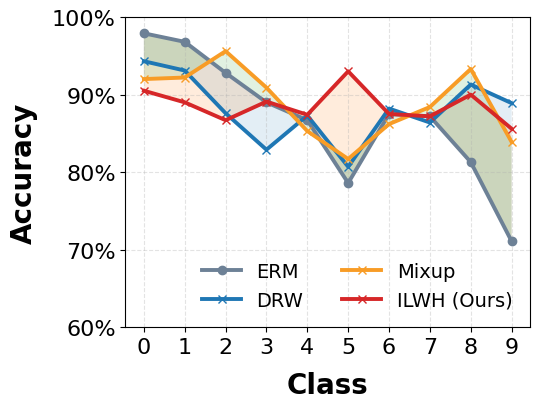
\includegraphics[width=\textwidth]{cinic_auto.png}
        \caption{Auto-aug -- CINIC-10}
        % \vspace{-7pt}
        \label{fig:cinic_auto}
    \end{subfigure}
    \begin{subfigure}[b]{0.30\textwidth}
        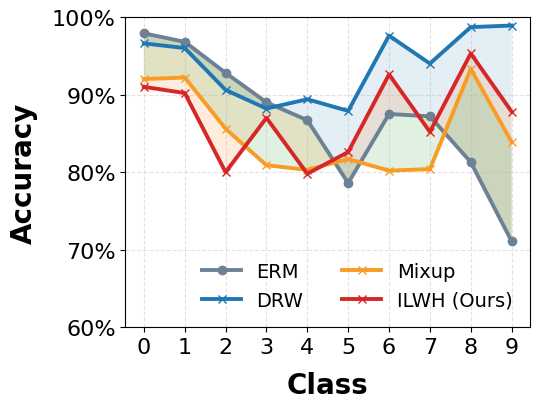
\includegraphics[width=\textwidth]{cinic_cutout.png}
        \caption{Cutout -- CINIC-10}
        % \vspace{-7pt}
        \label{fig:cinic_cutout}
    \end{subfigure}
    \begin{subfigure}[b]{0.30\textwidth}
        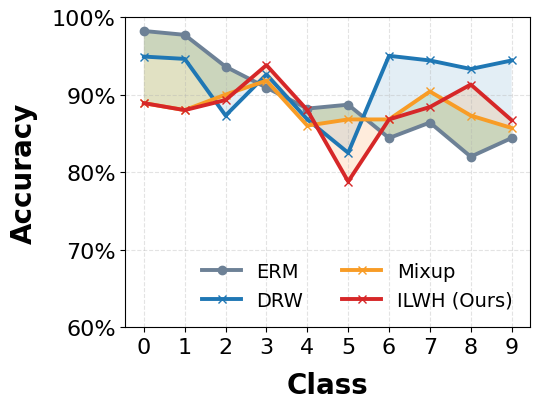
\includegraphics[width=\textwidth]{cinic10_rand.png}
        \caption{Rand-aug -- CINIC-10}
        % \vspace{-7pt}
        \label{fig:cinic10_rand}
    \end{subfigure}
    \begin{subfigure}[b]{0.30\textwidth}
        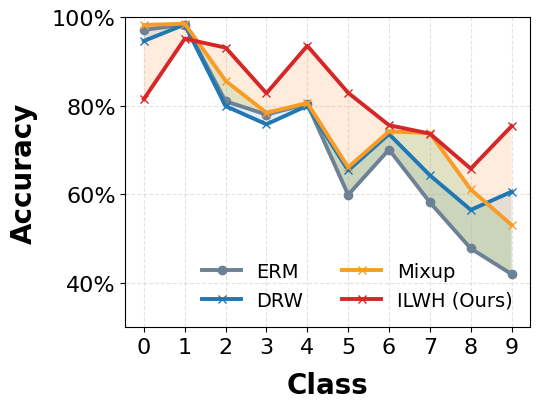
\includegraphics[width=\textwidth]{cifar10_auto.png}
        \caption{Auto-aug -- CIFAR-10}
        % \vspace{-7pt}
        \label{fig:cifar10_auto}
    \end{subfigure}
    \begin{subfigure}[b]{0.30\textwidth}
        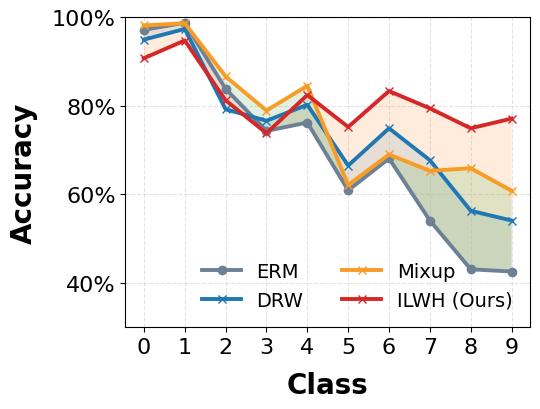
\includegraphics[width=\textwidth]{cifar10_cutout.png}
        \caption{Cutout -- CIFAR-10}
        % \vspace{-7pt}
        \label{fig:cifar10_cutout}
    \end{subfigure}
    \begin{subfigure}[b]{0.30\textwidth}
        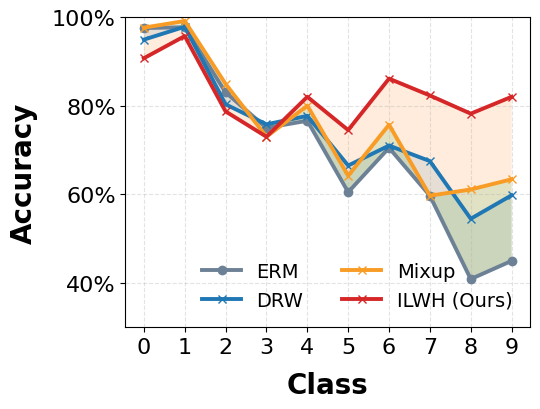
\includegraphics[width=\textwidth]{cifar10_randaug.png}
        \caption{Rand-aug -- CIFAR-10}
        % \vspace{-7pt}
        \label{fig:cifar10_randaug}
    \end{subfigure}
        \begin{subfigure}[b]{0.30\textwidth}
        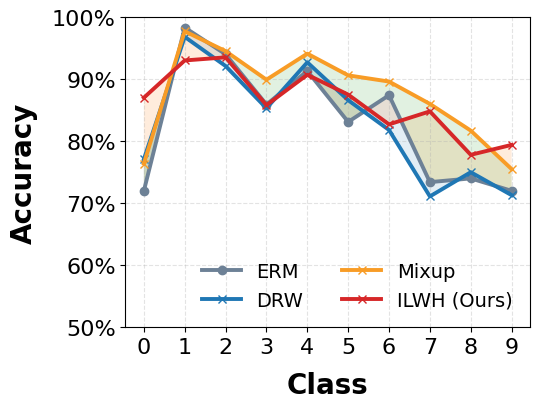
\includegraphics[width=\textwidth]{svhn_auto.png}
        \caption{Auto-aug -- SVHN-10}
        % \vspace{-7pt}
        \label{fig:svhn_auto}
    \end{subfigure}
    \begin{subfigure}[b]{0.30\textwidth}
        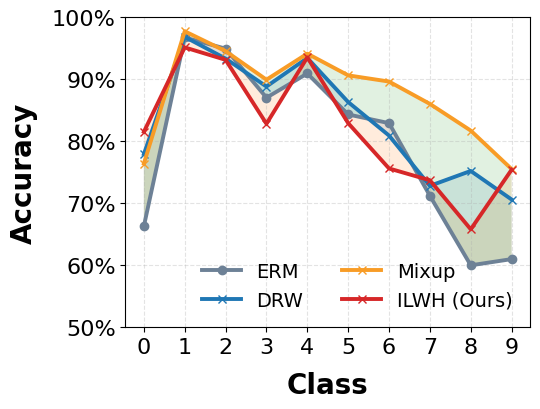
\includegraphics[width=\textwidth]{svhn_cutout.png}
        \caption{Cutout -- SVHN-10}
        % \vspace{-7pt}
        \label{fig:svhn_cutout}
    \end{subfigure}
    \begin{subfigure}[b]{0.30\textwidth}
        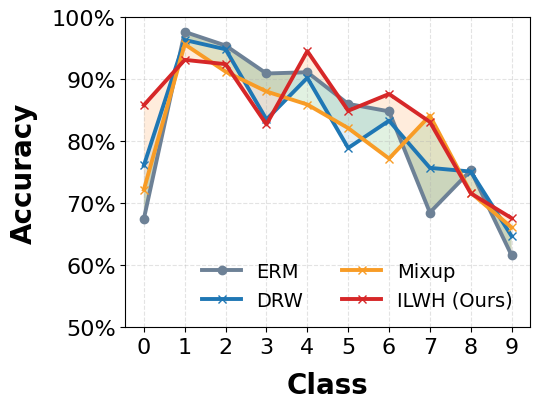
\includegraphics[width=\textwidth]{svhn_randaug.png}
        \caption{Rand-aug -- SVHN-10}
        % \vspace{-7pt}
        \label{fig:svhn_randaug}
    \end{subfigure}
    \caption{Comparison of per-class accuracy across different strategies, affected by different data augmentation methods. Proposed methods (\textit{DRW, Mixup, and ILWH}) consistently outperform ERM, with particularly large gains observed in minority (\textit{tail}) classes. This demonstrates that such sampling strategies not only improve overall accuracy but also enhance learning in underrepresented classes, addressing class imbalance more effectively.}
\end{figure*}

\textbf{Introducing Class Imbalance.} To evaluate our methods under imbalanced conditions, we artificially create long-tail imbalanced versions of the datasets. This was done consistently for all datasets using a fixed imbalance factor of 0.01. The process involves programmatically reducing the number of training samples per class according to the target exponential distribution. Specifically, for each class, we randomly selected a predetermined number of instances from the original dataset, discarding the remainder. For example, after this transformation, the training sample counts for the 10 classes in CIFAR-10 were set to \texttt{[5000, 2997, 1796, 1077, 645, 387, 232, 139, 83, 50]}, creating a controlled imbalanced environment for our experiments.
\begin{table*}[htb]
\centering
\caption{Computational complexity and training efficiency on CIFAR-10.}
\label{tab:complexity_cifar10}
\renewcommand{\arraystretch}{1.2}
\setlength{\tabcolsep}{1.2pt}
\begin{tabular}{lccccc}
\hline
 \textbf{Method} &\textbf{IwT} & \textbf{Avg FLOPs/Epo (G)} & \textbf{Total FLOPs (G)} & \textbf{Avg Time/Epo (s)} & \textbf{Rel. Cost} \\
\hline
M2m & \cmark & 6{,}589.37 & 1{,}317{,}873.27 & 6.32 & 1.00$\times$ \\
DeepSMOTE & \xmark & $\approx$9{,}884--13{,}179 & $\approx$1.98--2.64$\times 10^{6}$ & $\approx$9.5--12.6 & $\approx$1.5--2.0$\times$ \\
ILWH (Ours) & \cmark & 6{,}589.37 & 1{,}317{,}873.27 & \textbf{5.03} & \textbf{0.80$\times$} \\
\hline
\end{tabular}
\begin{tablenotes}
    \item \textit{\textbf{Integrate within Training (IwT)}}: \textit{The data augmentation process is generated within training progress. DeepSMOTE generates synthetic data before starting the training progress.}
\end{tablenotes}
\end{table*}

\textbf{Classification model.}
All methods use an identical ResNet-32 \cite{he2016deep} as their base classifier.

\textbf{Configuration.}
The training process involved the baseline data augmentation, where each image was padded by 4 pixels on each side, followed by a random 32 × 32 crop from the padded image or its horizontally flipped version. The model was trained for 200 except for TinyImageNet-200 in which it was trained for 300 epochs. The learning rate was initially set to 0.1 and decayed by a factor of 0.01. Additionally, a linear warm-up strategy was applied for the first 5 epochs to stabilize training and ensure a fair comparison~\cite{goyal2017accurate}. 

\textbf{Training Mode.}
The experiments were carried out using four training strategies: using ERM as a loss function, DRW, Mixup and our proposed ILWH.

\textbf{Performance Metrics.}
Performance is measured through metrics such as group accuracy for many-shot, medium-shot, and low-shot classes, confusion matrix-derived class recall, \textit{precision@1} and \textit{precision@5} for top predictions, and average loss tracking.

\subsection{Data Augmentation Experiment}
In our experimental evaluation, specific settings were adopted for each of the data augmentation techniques to ensure reproducibility and align with common practices.

For \textit{AutoAugment}, we employed the predefined and appropriate policies learned for each specific dataset to guide the augmentation. For CIFAR-10, CIFAR-100, and CINIC-10, we used the \texttt{AutoAugmentPolicy.CIFAR10}. This single policy is suitable for all three as they share similar image characteristics and content domains. For the SVHN-10 dataset, we applied its specifically trained \texttt{AutoAugmentPolicy.SVHN}. Similarly, for experiments involving Tiny-ImageNet-200, we utilized the \texttt{AutoAugmentPolicy.ImageNet}, which was originally discovered on the full ImageNet dataset. This approach ensures that the augmentation strategies are well-suited to the underlying distribution of each dataset.
\begin{figure*}[htb]
    \centering
    \begin{subfigure}[b]{1.0\textwidth}
        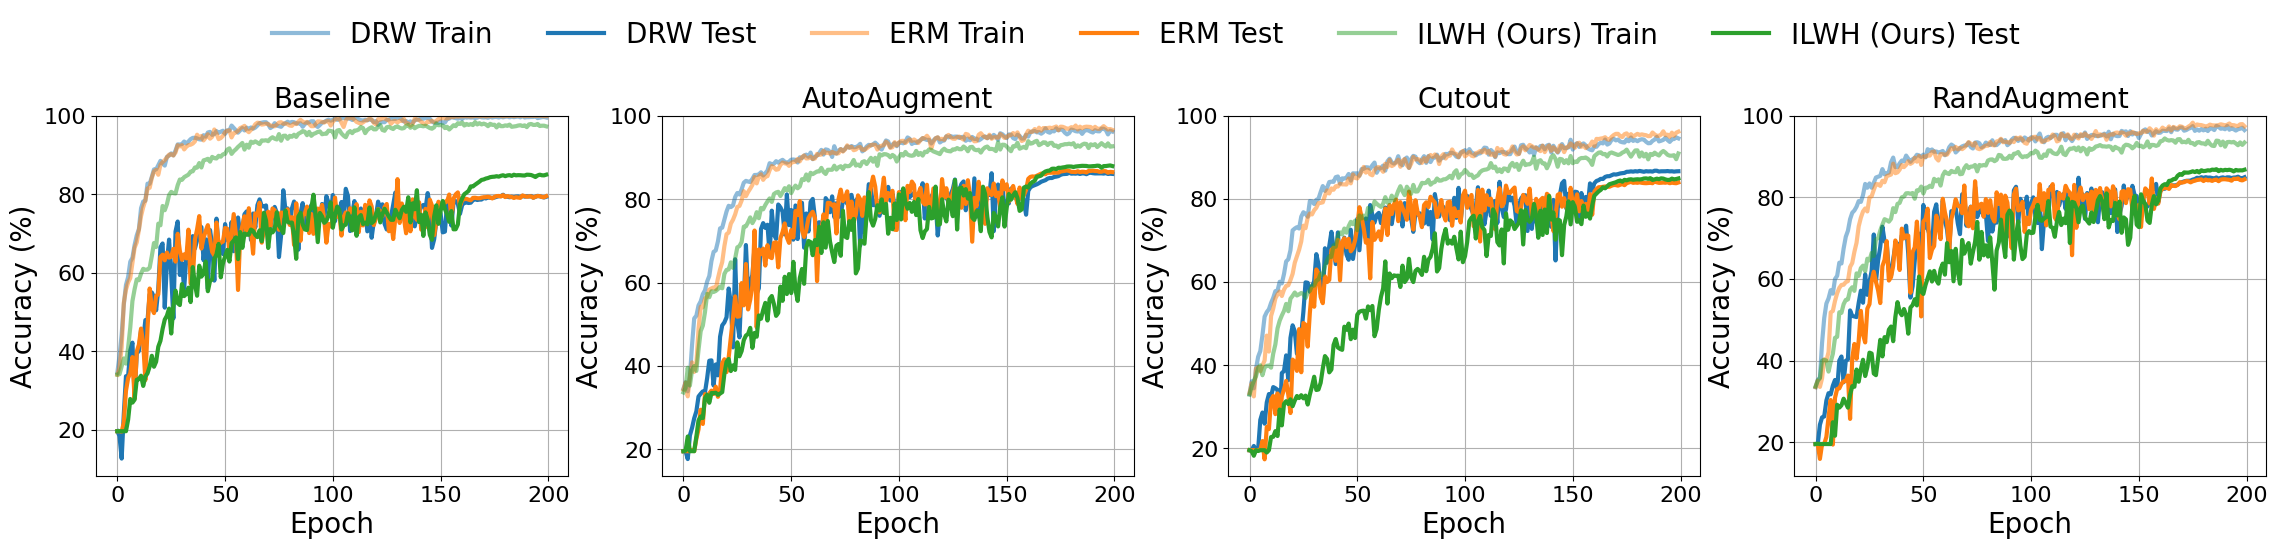
\includegraphics[width=\textwidth]{svhn_exp.png}
        % \caption{SVHN}
        \vspace{-5pt}
        \label{fig:svhn_exp}
    \end{subfigure}
    \begin{subfigure}[b]{1.0\textwidth}
        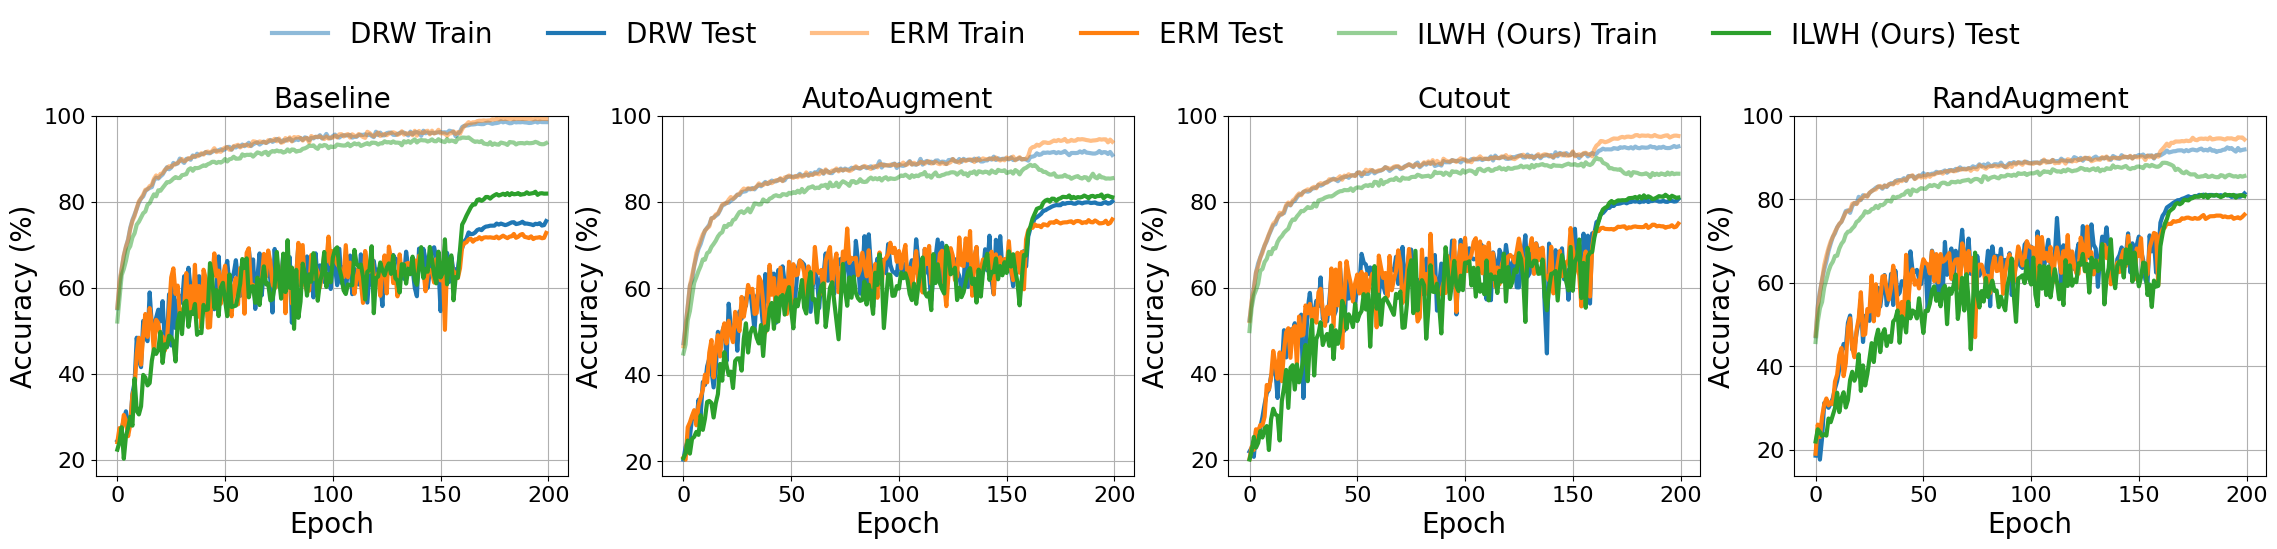
\includegraphics[width=\textwidth]{cifar10_exp.png}
        % \caption{CIFAR-10}
        \vspace{-5pt}
        \label{fig:cifar10_exp}
    \end{subfigure}
    \begin{subfigure}[b]{1.0\textwidth}
        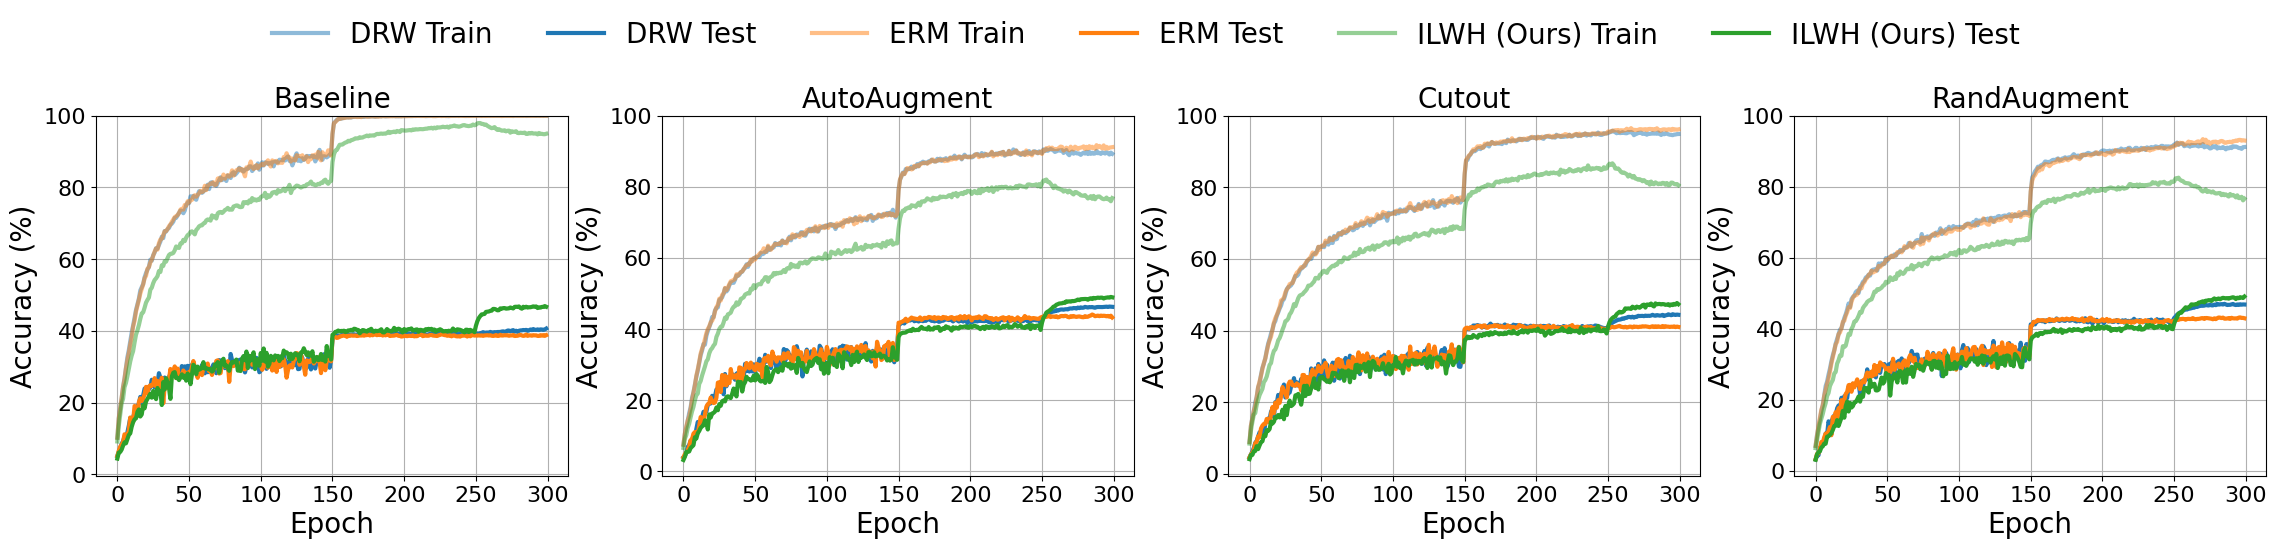
\includegraphics[width=\textwidth]{cifar100_exp.png}
        % \caption{CIFAR-100}
        \vspace{-5pt}
        \label{fig:cifar100_exp}
    \end{subfigure}
    \caption{Training and testing accuracy curves on SVHN-10 (\textbf{top}), CIFAR-10 (\textbf{middle}) and CIFAR-100 (\textbf{bottom}) with different data augmentation methods.}
\end{figure*}

Regarding \textit{RandAugment}, which offers a simplified approach to automated augmentation, we set its two primary hyperparameters as follows: the number of augmentation transformations to apply sequentially, $N$, was chosen as 2, and the global magnitude for these transformations, $M$, was set to 14. These values were selected based on common settings that balance augmentation strength and computational efficiency.

For the \textit{Cutout} regularization technique, our experiments involved applying a randomly positioned square mask of size $16 \times 16$ pixels to the input images during training. This size was chosen to introduce a moderate level of occlusion, encouraging the model to learn more distributed features.

\subsection{Data Sampling Experiment}

For our main comparative experiments, we fixed this parameter to \(\alpha=0.5\) across all datasets to maintain a consistent and moderate level of balancing. It is important to note that this sampling process occurs after the data augmentation transformation. These sampling strategies were integrated directly into the training pipeline by passing a custom batch sampler to the \texttt{DataLoader}. This ensures that each mini-batch is constructed according to the specified sampling logic, rather than simple sequential or random sampling over the entire dataset.

\subsection{Computational Efficiency Analysis}

We evaluated the computational complexity of each method using the ptflops package and measured wall-clock training time. As shown in Table \ref{tab:complexity_cifar10}, \textbf{ILWH (Ours)} requires FLOPs identical to the M2m baseline (6.59 × 10³ G per epoch) but reduces average epoch time by approximately 20\% . In contrast, \textbf{DeepSMOTE} introduces substantially higher computational overhead ($\sim$1.5--2$\times$) due to its encoder-decoder generation module, which increases both forward- and backward-pass costs. This analysis confirms that the proposed \textbf{ILWH (Ours)} design maintains computational efficiency while improving performance on imbalanced data, while generative oversampling approaches like DeepSMOTE trade efficiency for synthetic diversity \cite{dablain2022deepsmote}.

\subsection{Result Analysis}
According  to the results in  Table \ref{tab:drw_results_cifar_svhn_cinic} and Table \ref{tab:drw_results_cifar100_tiny}, the overall performance of  ILWH achieved effectiveness across different  datasets when compared to introduced methods. To be precise in Table  \ref{tab:drw_results_cifar_svhn_cinic}, our methodology has outperformed the other ones with \textbf{top 1 Accuracy} when conducted on common augmentations and several samplings. It is a strong  evidence that our research potentially can optimize not only computing-resources but also overall model performances. Despite these promising results on datasets with less complex patterns and smaller sample sizes (\textit{e.g., CIFAR-10, SVHN-10, CINIC-10}), the performance on the more challenging CIFAR-100 and TinyImageNet-200 datasets remains at a tolerable level. Post-training accuracies for these complex tasks generally range from 30\% to nearly 50\%. Nevertheless, as reflected in the aforementioned tables, our research not only introduces an innovative approach to address this ingrained problem but also offers a promising direction for future AI researchers to achieve higher performance without the need for intensive computational resources.

The experimental results presented in Figures \ref{fig:drw_affect}, \ref{fig:comparision_m2m_deepSMOTE_Ours}, and \ref{fig:weight_dist} collectively demonstrate the effectiveness of the proposed lightweight imbalanced learning method. As shown in Figure \ref{fig:drw_affect}, applying the DRW strategy after the $160^{th}$ epoch leads to a significant reduction in both training and testing losses. Before applying DRW, the model experiences a slower decline in loss, indicating that it is learning general features without being overly influenced by class imbalance. However, once DRW is introduced, the loss curves drop sharply, suggesting that the model benefits from the delayed application of class weight. This delayed balancing allows the model to first learn stable representations and then focus on minority classes later in training, thereby improving convergence stability and generalization performance.

Figure \ref{fig:comparision_m2m_deepSMOTE_Ours} further supports these findings by comparing the proposed method with other resource-intensive techniques such as M2m and DeepSMOTE on the CIFAR-10 and CIFAR-100 datasets. On CIFAR-10, the proposed approach achieves comparable accuracy to these heavy models while maintaining computational efficiency. Similarly, on CIFAR-100, it delivers competitive results, demonstrating that the combination of lightweight augmentations and DRW can achieve high accuracy without requiring complex architectures or extensive computational resources. This result confirms the strength of the proposed method in achieving a balance between efficiency and performance.

In Figure \ref{fig:weight_dist}, the normalized class weight distribution across training epochs provides insight into how DRW dynamically adjusts learning focus. At the beginning of training, the weight is almost uniform across classes, indicating that the model treats all samples equally. After DRW is activated at epoch $160^{th}$, the weight of minority classes gradually increases while those of majority classes remain stable or slightly decrease. This adaptive re-weighting ensures that underrepresented classes receive more attention in the later training stages, helping to mitigate class imbalance and improve recognition of rare categories.
\section{Conclusion} \label{sec:conclusion}

In this work, we evaluate lightweight strategies designed to address the challenges of imbalanced learning under limited computational resources. When resource constraints restrict the use of large-scale or computationally heavy models, achieving both efficiency and robustness becomes crucial. Our study systematically investigates how lightweight configurations behave when combined with data-level and training-level adjustments such as augmentation and DRW.

Although individual lightweight methods may not perform effectively when applied in isolation, we observe that combining them with data augmentation and DRW leads to consistent and stable improvements across multiple datasets. This reveals an important phenomenon: even under limited capacity, the synergy between balanced sampling and regularization through augmentation can significantly enhance model generalization.

Furthermore, our benchmark over five diverse datasets demonstrates that, when properly regularized, random-based lightweight approaches achieve surprisingly competitive performance among various sampling and combination strategies, including random sampling, weighted sampling, and hybrid augmentation setups. This highlights that simple yet well-calibrated lightweight pipelines can remain effective solutions in constrained environments.
\section{Limitation}

Despite the promising results of lightweight data augmentation techniques for handling imbalanced datasets, there are several limitations to consider in this study.

\paragraph{Limited exploration of extreme imbalance ratios} The experiments of this work primarily focus on relatively mild imbalances, with ratios up to 100:1. Further research is required to assess the effectiveness of these methods in scenarios with more extreme imbalances, such as those with 1000:1 or even higher class imbalances. 

\paragraph{Generalization to Large-Scale Multi-Class Datasets} While the methods demonstrated good results on datasets like SVHN-10, CIFAR-10, CINIC-10, CIFAR-100, and TinyImageNet-200 their performance on extremely large-scale datasets with a higher number of classes (\textit{e.g., datasets with thousands of classes, such as ImageNet}) remains underexplored. The computational efficiency of these techniques might degrade when scaled up, especially in resource-constrained environments.

\paragraph{Lack of Cross-Domain Validation}The study chiefly evaluates methods to the classical problem of image classification. It would be beneficial to extend the proposed techniques to other domains, such as text or speech recognition, where class imbalance manifests itself differently. This would allow for a broader understanding of the generalizability and adaptability of the proposed lightweight techniques.




\bibliographystyle{IEEEtran}
\bibliography{reference.bib}


\begin{IEEEbiography}[{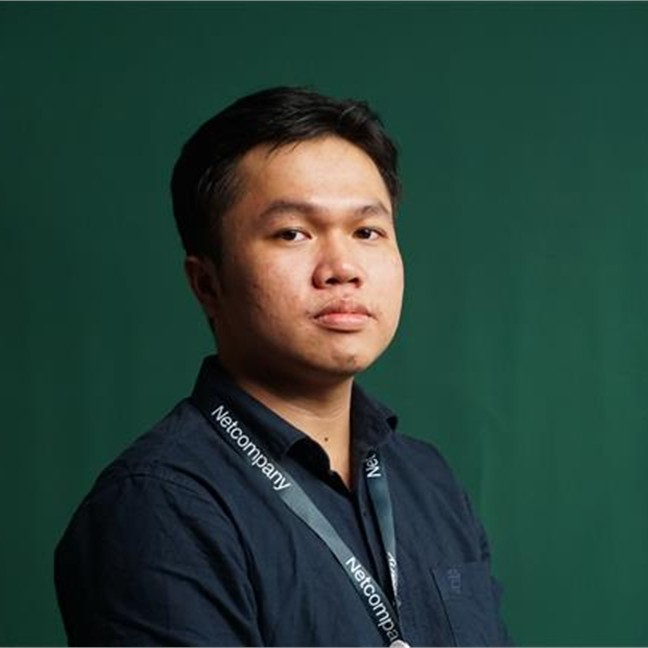
\includegraphics[width=1.1in,height=1.25in,clip,keepaspectratio]{dtd.jpg}}]{Thai-Duy Dinh}
received a double degree from Frankfurt University of Applied Sciences and the Vietnamese-German University. He was recognized with a National Mathematics Award for university students, earning a Silver Medal in Algebra and a Bronze Medal in Calculus. His thesis includes mosquito classification, audio signal processing, and machine learning applications. He has pursued work in imbalanced data learning, weakly supervised learning, and optimal transport. Also, he is currently working as an IT Consultant at Netcompany.
% \vspace{-5\baselineskip}
\end{IEEEbiography}

\begin{IEEEbiography}[{
\includegraphics[width=1.1in,height=1.25in,clip,keepaspectratio]{thuan.jpg}}]{Minh-Thuan Nguyen}
was born in Ho Chi Minh City, Vietnam, he received a double degree from Frankfurt University of Applied Sciences and the Vietnamese-German University. His thesis involved collecting large-scale job-posting data and analyzing it with large language model (LLM) methods. He developed machine-learning models for a priority voice-routing dataset used in telecommunications. He is currently a member of the AAIR Lab at the Vietnamese-German University, where research focuses on imbalanced learning, machine learning, AI vision, applications of LLMs, and weakly-supervised learning.
% \vspace{-5\baselineskip}
\end{IEEEbiography}

\begin{IEEEbiography}
[{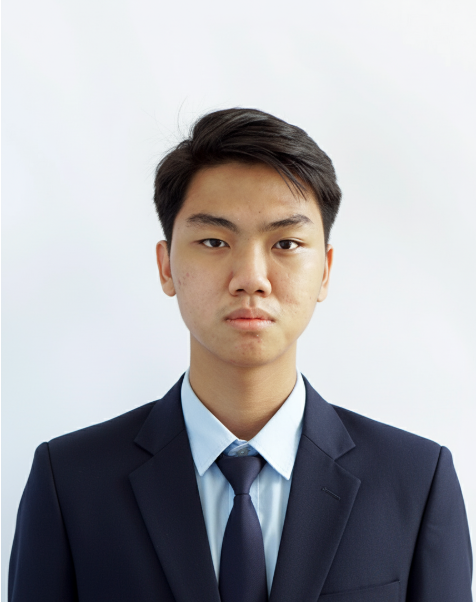
\includegraphics[width=1.1in,height=1.25in,clip,keepaspectratio]{kim.png}}]{Thanh-Kim Le Duc }
was born in Ho Chi Minh City, Vietnam, and is currently a final-year student at the Vietnamese-German University. He is a member of the AAIR Lab at the Vietnamese-German University, where his research focuses on imbalanced learning and semi-supervised learning, with applications in robust and efficient machine learning. His academic work emphasizes developing methods that address data scarcity and distributional imbalance, aiming to improve generalization and fairness in real-world scenarios.
\end{IEEEbiography}

\begin{IEEEbiography}
[{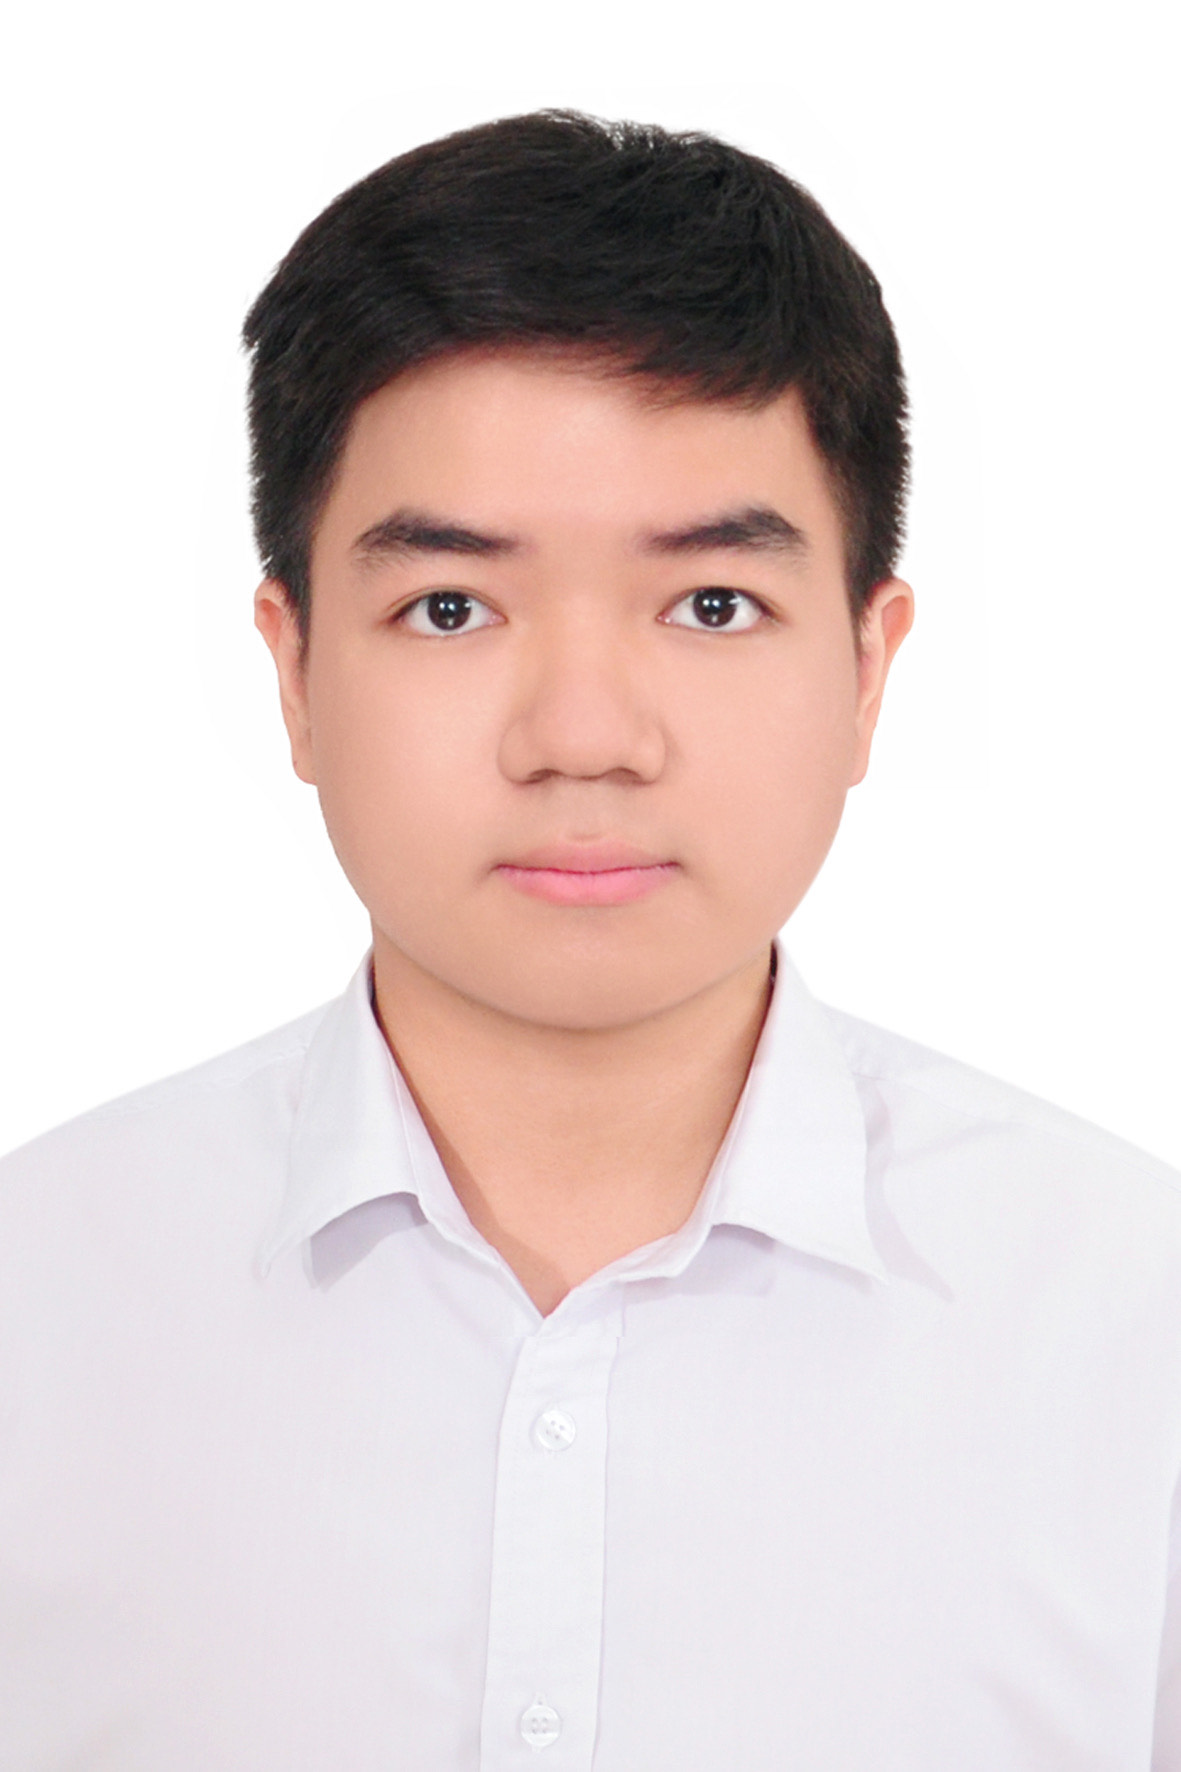
\includegraphics[width=1.1in,height=1.25in,clip,keepaspectratio]{dat.jpeg}}]{Man-Dat Nguyen}
was born in Ho Chi Minh City, Vietnam. He received a double degree from Frankfurt University of Applied Sciences and the Vietnamese-German University. His interests include imbalanced data learning, lightweight machine learning, and efficient training strategies for real-world applications. He has worked on mosquito classification and on-device AI systems, with particular interest in data augmentation and effective re-weighting methods for imbalanced classification.
% \vspace{-5\baselineskip}
\end{IEEEbiography}

\begin{IEEEbiography}[{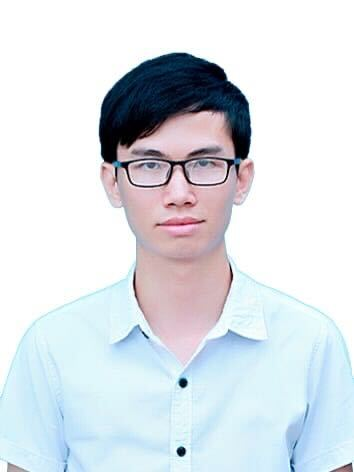
\includegraphics[width=1.1in,height=1.25in,clip,keepaspectratio]{quang.jpg}}]{Duc-Quang Vu} received the Ph.D. degree in Department of Computer Science \& Information Engineering, National Central University, Taiwan in 2022. He is currently a lecturer at Thai Nguyen University of Information and Communication Technology and a researcher at Queen's University of Belfast.
He receives several awards and honors, including 2nd in the National Informatics Olympiad for Universities, Vietnam in 2009; 3rd in National Informatics Olympiad for Universities, Vietnam in 2011; 4th in the Young Scientist Talent Contest for Universities, Vietnam in 2012. He currently a reviewer at several journals and conferences such as Multimedia Systems, Engineering Applications of Artificial Intelligence, ECAI, ACML, etc. His research interests include machine learning, deep learning, computer vision, and bioinformatics.
% \vspace{-5\baselineskip}
\end{IEEEbiography}

\begin{IEEEbiography}
[{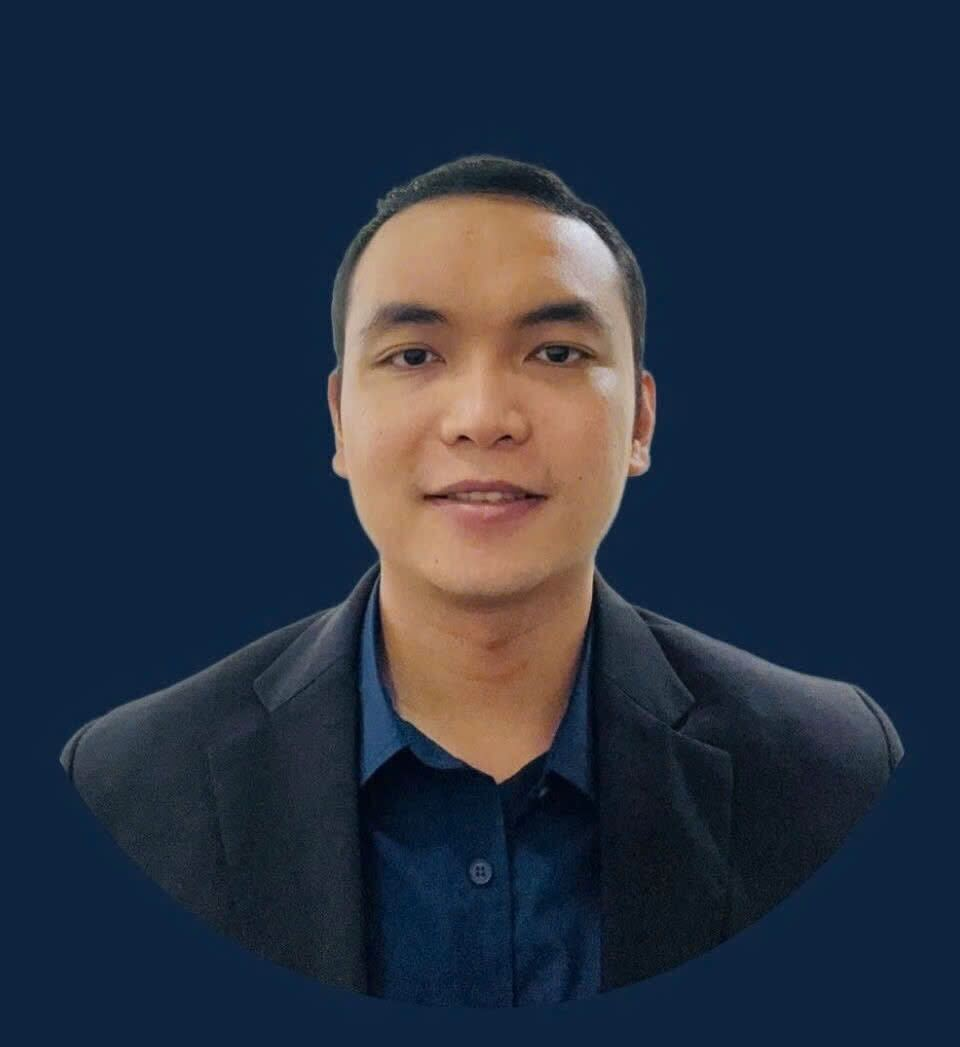
\includegraphics[width=1.1in,height=1.15in,clip,keepaspectratio]{TNH.jpg}}]{Ngoc-Hoang Tran} received the B.S. degree in mechatronics engineering from the Ho Chi Minh City University of Technology, Ho Chi Minh City, Vietnam, in 2015, and the Ph.D. degree in electrical and computer engineering from Sungkyunkwan University, Suwon, South Korea, in 2020.
From 2020 to 2022, he was a Postdoctoral Researcher with the Department of Electrical and Computer Engineering, Sungkyunkwan University. Since 2022, he has been a Lecturer and a Researcher with the Department of Software Engineering, FPT University, Can Tho, Vietnam. His research interests include signal processing, motion control, embedded systems, autonomous robotics, computer vision, machine learning, and deep learning.
% \vspace{-5\baselineskip}
\end{IEEEbiography}

\begin{IEEEbiography}
[{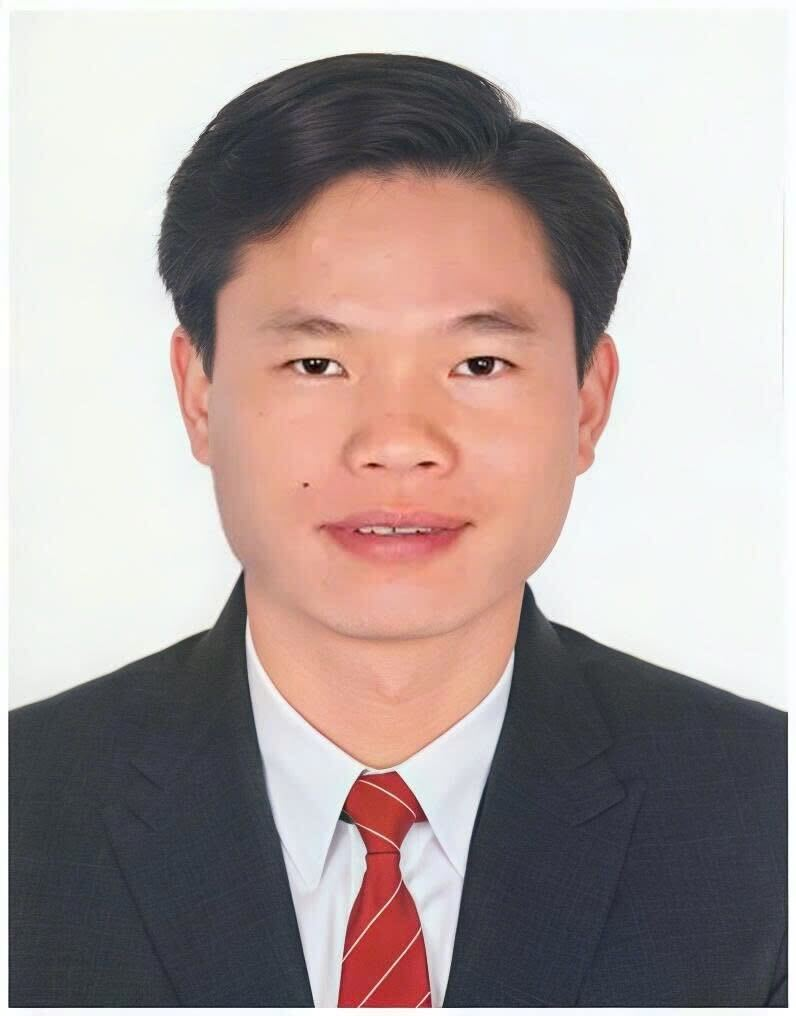
\includegraphics[width=1.15in,height=1.25in,clip,keepaspectratio]{PAC.jpg}}]{Anh-Cang Phan} is a lecturer at Vinh Long University of Technology Education, Vietnam. He received his Ph.D. in Informatics from Aix-Marseille University, France, and was conferred the title of Associate Professor in 2023. His research interests cover a range of topics, including Machine Learning, Deep Learning, Big Data, IoT and 3D Modeling, with a strong focus on developing intelligent systems that bridge the gap between theory and real-world applications. Over the years, Dr. Phan has conducted numerous practical and interdisciplinary research projects, particularly in smart agriculture, intelligent irrigation systems, and medical image processing applications that have been successfully implemented in several hospitals across Vietnam. His works contribute significantly to advancing digital transformation in both the agricultural and healthcare sectors. In 2020, Dr. Phan was listed in the Vietnam Yellow Book of Innovation by the Ministry of Science and Technology, recognizing his outstanding contributions to scientific research, innovation, and technological development in Vietnam.
\end{IEEEbiography}

\begin{IEEEbiography}
[{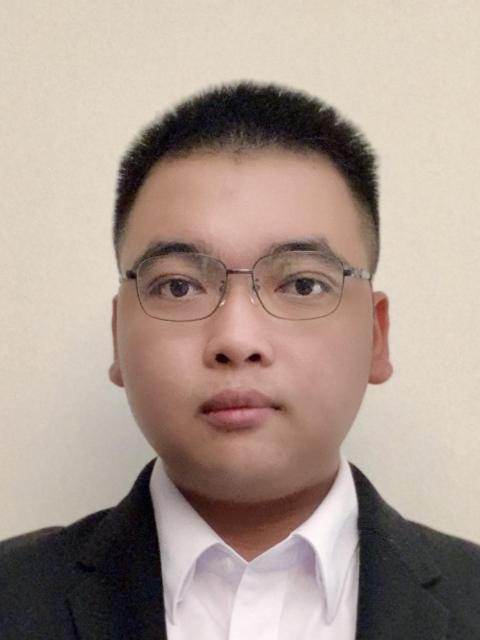
\includegraphics[width=1.1in,height=1.25in,clip,keepaspectratio]{LNH.jpg}}]{Ngoc-Hoang Le} M.Sc. is currently a Ph.D. student at the Graduate Institute of Biomedical Materials and Tissue Engineering, College of Biomedical Engineering, Taipei Medical University, Taiwan. He received his Master’s degree in Biomedical Materials and has been actively engaged in interdisciplinary research at the interface of biomedical materials, nanotechnology, and artificial intelligence in medicine. His current work focuses on the development of advanced bio/nanomaterials for ocular and musculoskeletal applications, as well as the design of AI-driven pipelines for medical image analysis and translational healthcare.
\end{IEEEbiography}

\begin{IEEEbiography}
[{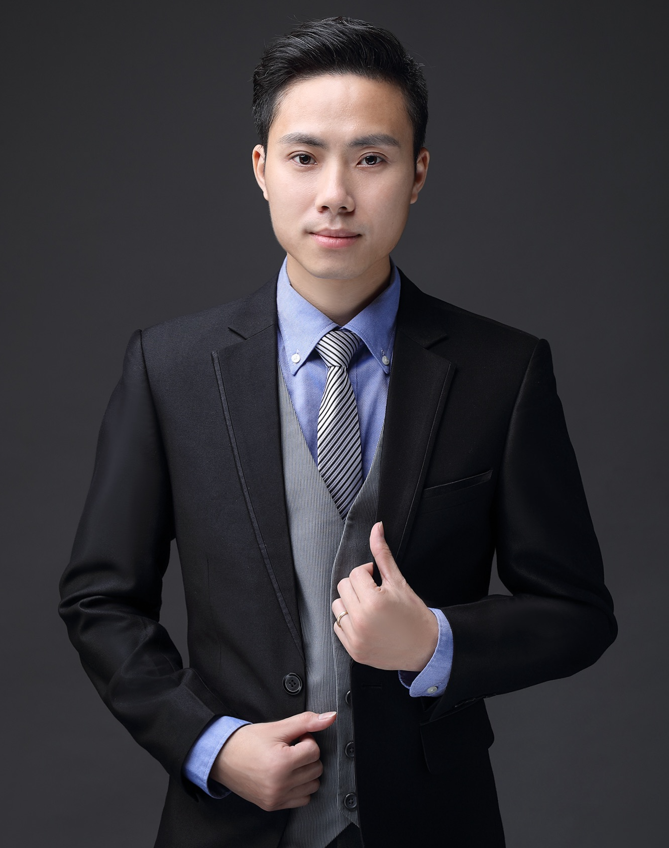
\includegraphics[width=1.1in,height=1.15in,clip,keepaspectratio]{PA.png}}]{Phung-Anh Nguyen} currently works as an assistant professor at Graduate Institute of Data Science in Taipei Medical University with expertise in medical informatics, data analytics, machine learning, and human-computer interaction, focus on the life science.
He hold a Bachelor of Engineering of Science (Major in Information Technology) from Hanoi Open University, Hanoi, Vietnam. Afterward, 
he graduated as Doctor of Philosophy (Ph.D.) in Biomedical Informatics at National Yang-Ming University, Taipei, Taiwan. Among 10 years of experiences in the field of Healthcare Informatics, he has developed the HIT products and implemented the HIT projects for clients who are from enterprise to ministry. Project scope has been covered in different levels (from small to huge; from enterprise to national level), and it is defined in fields as ICT, Healthcare. Especial, he has a lot of lessons learned when he have faced the difficult matters of the project in several roles (engineering, researcher, manager, and so forth). It is valued experiences to help me to manage projects successfully.
    % \vspace{-5\baselineskip}
\end{IEEEbiography}

\begin{IEEEbiography}
[{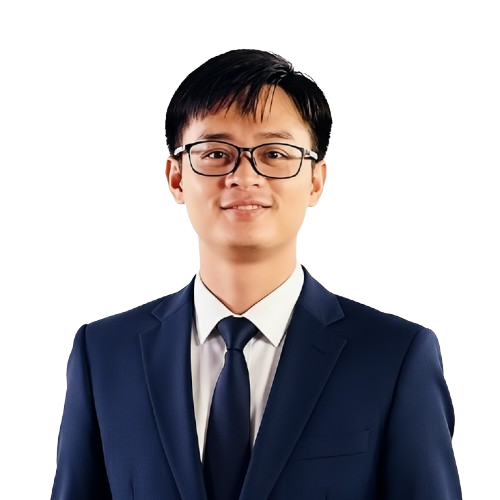
\includegraphics[width=1.15in,height=1.25in]{mth.png}}]{Tan-Ha Mai}
is a PhD candidate in Computer Science and Information Engineering at National Taiwan University. His research focuses on weakly supervised and imbalanced learning, optimal transport, large language models (LLMs), vision–language models (VLMs), and semi-supervised learning, with particular emphasis on developing practical and robust methods for complementary-label learning (CLL). He brings over a decade of industry experience in managing cloud infrastructure, telephony solutions, AI projects, and DevOps operations for Swiss and Japanese companies. Combining research and industry expertise, he is dedicated to inspiring future innovators as a lecturer. Ha has served as Workflow Chair and Session Chair for ACML 2024, and as a reviewer for leading AI conferences and journals, including AISTATS, TPAMI, ACML, AAAI, NeurIPS and CVPR.
% \vspace{-20\baselineskip}
\end{IEEEbiography}

\begin{IEEEbiography}
[{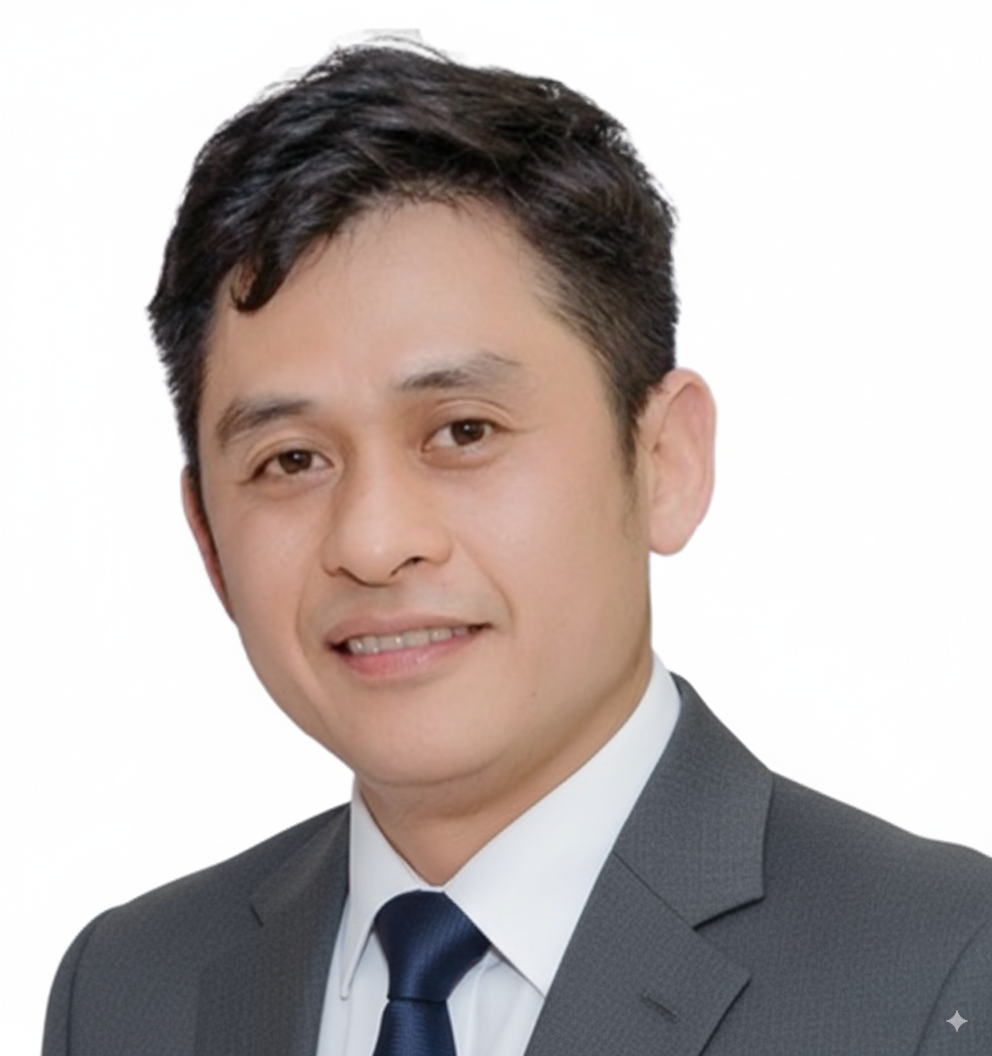
\includegraphics[width=1.1in,height=1.25in,clip,keepaspectratio]{LLSon.png}}]{Lam-Son L\^{e}}
(Member, IEEE) received his Ph.D. from the \'{E}cole Polytechnique F\'{e}d\'{e}rale de Lausanne, Switzerland, in 2008. He spent four years as a Postdoctoral Researcher at the University of Wollongong, Australia. He currently holds dual roles at the Vietnamese-German University: Academic Coordinator of the Bachelor's program in Computer Science and Lecturer in Software Engineering. His research interests include digital twins, decentralized computing, next-generation software architectures, and AI-driven business process management. Prior to joining VGU, he spent nine years at the Ho Chi Minh City University of Technology (HCMUT) -- Vietnam National University, where he led a research group focused on data-driven enterprise software and processes. Lam-Son has successfully supervised three PhD students, served as program chair, demo track chair, publicity chair for various conferences in software engineering and enterprise computing. He has published around 70 papers in conference proceedings and journals.
% \vspace{-5\baselineskip}
\end{IEEEbiography} 

%The first paragraph may contain a place and/or date of birth (list place, then date). Next, the author's educational background is listed. The degrees should be listed with type of degree in what field, which institution, city, state, and country, and year the degree was earned. The author's major field of study should be lower-cased. 

%The second paragraph uses the pronoun of the person (he or she) and not the author's last name. It lists military and work experience, including summer and fellowship jobs. Job titles are capitalized. The current job must have a location; previous positions may be listed without one. Information concerning previous publications may be included. 
\EOD
\end{document}

